%=====================================================================
% BÀI BÁO KHOA HỌC — ĐỀ XUẤT KIẾN TRÚC THAM CHIẾU, VJST-MOST
% Định dạng ưu tiên theo mẫu biên tập 4044_VJST.docx và quy định chi tiết VJST.
%=====================================================================
\documentclass[a4paper,12pt]{article}

\usepackage{fontspec}
\IfFontExistsTF{Times New Roman}
  {\setmainfont{Times New Roman}[Ligatures=TeX]}
  {\setmainfont{DejaVu Serif}[Ligatures=TeX]}
\usepackage{polyglossia}
\setmainlanguage{vietnamese}
\setotherlanguage{english}

% Quy định chi tiết VJST: A4, lề trên/dưới 2 cm, trái 3 cm, phải 2 cm.
% Mẫu biên tập 4044 dùng thân chữ 13 pt và giãn dòng 1,2.
\usepackage[a4paper,top=2cm,bottom=2cm,left=3cm,right=2cm]{geometry}
\usepackage{graphicx}
\usepackage{booktabs}
\usepackage{tabularx}
\usepackage{longtable}
\usepackage{multirow}
\usepackage{array}
\usepackage{caption}
\usepackage{float}
\usepackage{enumitem}
\usepackage{amsmath,amssymb}
\usepackage{xcolor}
\usepackage{tikz}
\usetikzlibrary{arrows.meta,positioning,fit,calc,shapes.geometric}
\usepackage{setspace}
\usepackage{titlesec}
\usepackage[hidelinks]{hyperref}
\usepackage[english]{cleveref}
\usepackage[numbers,sort&compress]{natbib}

% Thân chữ 13 pt như bản 4044_VJST.docx.
\AtBeginDocument{\fontsize{13pt}{15.6pt}\selectfont}
\setstretch{1.2}
\setlength{\parindent}{1.27cm}
\setlength{\parskip}{3pt}
\emergencystretch=2em
\setlist{nosep,leftmargin=*}

% Tiêu đề mục trong bản 4044 giữ cùng cỡ thân bài, in đậm.
\titleformat{\section}{\bfseries\fontsize{13pt}{15.6pt}\selectfont}{\thesection.}{0.45em}{}
\titleformat{\subsection}{\bfseries\fontsize{13pt}{15.6pt}\selectfont}{\thesubsection.}{0.45em}{}
\titleformat{\subsubsection}{\bfseries\fontsize{13pt}{15.6pt}\selectfont}{\thesubsubsection.}{0.45em}{}
\titlespacing*{\section}{0pt}{6pt}{3pt}
\titlespacing*{\subsection}{0pt}{5pt}{2pt}
\titlespacing*{\subsubsection}{0pt}{4pt}{2pt}

\DeclareCaptionFont{vjstcaption}{\fontsize{13pt}{15.6pt}\selectfont}
\captionsetup{font=vjstcaption,labelfont=bf,textfont=bf,labelsep=period}
\renewcommand{\refname}{TÀI LIỆU THAM KHẢO}

% Ghi chú nội bộ: giữ trong source nhưng ẩn ở PDF bản sạch.
\newcommand{\note}[1]{\textcolor{red}{\small[GHI CHÚ: #1]}}
\renewcommand{\note}[1]{}

\newcommand{\vjsttablefont}{\fontsize{10pt}{12pt}\selectfont}
\newcommand{\dnkhcn}{DN KH\&CN}
\newcommand{\dnknst}{DN KNST}
\newcommand{\khcn}{KH\&CN}
\newcommand{\dmst}{ĐMST}

\begin{document}
%=====================================================================
% 00 — THÔNG TIN ĐẦU BÀI THEO MẪU BIÊN TẬP 4044_VJST
% Tác giả/cơ quan giữ nguyên theo bản 4044_VJST.docx.
% Các mốc received/revised/accepted không được tự điền ở bản nộp mới.
%=====================================================================

\begin{center}
{\bfseries
Kiến trúc tham chiếu tỉnh--trung ương cho nền tảng số quản lý doanh nghiệp khoa học và công nghệ và doanh nghiệp khởi nghiệp sáng tạo\par}
\vspace{0.45em}
{\bfseries Nguyễn Đình Quảng\textsuperscript{1}, Nguyễn Huy Cường\textsuperscript{2*}\par}
\vspace{0.35em}
{\itshape
\textsuperscript{1}Khoa Công nghệ thông tin, Học viện Công nghệ Bưu chính viễn thông,\\
96A Trần Phú, phường Hà Đông, Hà Nội, Việt Nam\par}
\vspace{0.2em}
{\itshape
\textsuperscript{2}Trung tâm Phát triển doanh nghiệp khoa học và công nghệ, Cục Khởi nghiệp và Doanh nghiệp công nghệ, Bộ Khoa học và Công nghệ, 115 Trần Duy Hưng, phường Yên Hòa, Hà Nội, Việt Nam\par}
\end{center}

% Ngày nhận/chuyển phản biện/chấp nhận đăng do Tòa soạn bổ sung ở giai đoạn biên tập.
\begingroup
\renewcommand{\thefootnote}{*}
\footnotetext{\textit{Tác giả liên hệ: Email: nguyenhuycuong@mst.gov.vn}}
\endgroup

%=====================================================================
% 01 — TÓM TẮT VI + EN — WP6 compressed
%=====================================================================

\noindent\textbf{\textit{Tóm tắt:}}

\noindent
\textbf{Quản lý doanh nghiệp khoa học và công nghệ (DN KH\&CN) và doanh nghiệp khởi nghiệp sáng tạo (DN KNST) chủ yếu thuộc thẩm quyền cấp tỉnh nhưng cần liên thông và tổng hợp ở cấp trung ương. Theo nghiên cứu khoa học thiết kế (\textit{Design Science Research}, DSR), nghiên cứu đề xuất một kiến trúc tham chiếu phần mềm (SRA) tỉnh--trung ương có khả năng truy vết. Phát hiện trung tâm là quyền ghi cần được biểu diễn như một gán có phạm vi thẩm quyền và thời gian hiệu lực, không phải một thuộc tính địa bàn tĩnh, với một máy trạng thái năm bước bảo toàn bất biến một writer hợp lệ tại một thời điểm (single-active-writer). SRA tách lõi ổn định khỏi các điểm biến thiên, xác định nguồn dữ liệu theo nhóm thuộc tính, đồng thời quản trị cấu hình quy trình và liên thông mà không khóa cấu trúc lưu trữ vật lý. Mười kịch bản trước triển khai phát hiện hai khoảng trống: chuyển quyền ghi theo thời gian và khả năng cùng tồn tại của các phiên bản khác nhau. Sau tinh chỉnh, cùng rubric cho kết quả 2 kịch bản đáp ứng trực tiếp, 8 đáp ứng có điều kiện và không còn rủi ro kiến trúc chưa được hấp thụ ở mức L2. Các kết quả được cô đọng thành ba nguyên tắc thiết kế có khả năng chuyển giao cho các nền tảng chính phủ đa cấp khác: phân rã thẩm quyền theo nhóm thuộc tính--phạm vi--thời gian; tách lõi pháp lý ổn định khỏi biến thể vận hành; và duy trì provenance/liên thông độc lập với topology lưu trữ. Đây là kiểm chứng kiến trúc dựa trên kịch bản, không phải bằng chứng thực nghiệm; nguyên mẫu vẫn cần kiểm thử chuyển quyền, nâng cấp, liên thông, phục hồi, an toàn và các thuộc tính chất lượng đo được.}

\vspace{0.4em}
\noindent\textbf{\textit{Từ khóa:}} \textbf{doanh nghiệp khoa học và công nghệ, kiến trúc dữ liệu, kiến trúc tham chiếu, khởi nghiệp sáng tạo, liên thông hệ thống, quy trình cấu hình.}

\vspace{0.2em}
\noindent\textbf{\textit{Chỉ số phân loại:}} \textbf{1.2, 2.2}

\newpage
\begin{english}
\begin{center}
{\bfseries A provincial--central reference architecture for a digital platform managing science and technology enterprises and innovative startups\par}
\vspace{0.4em}
{\bfseries Dinh Quang Nguyen\textsuperscript{1}, Huy Cuong Nguyen\textsuperscript{2*}\par}
\vspace{0.3em}
{\itshape \textsuperscript{1}Faculty of Information Technology, Posts and Telecommunications Institute of Technology, 96A Tran Phu Street, Ha Dong Ward, Hanoi, Vietnam\par}
\vspace{0.15em}
{\itshape \textsuperscript{2}Technology and Science Enterprise Development Center, National Agency for Technology Entrepreneurship and Commercialization, Ministry of Science and Technology, 115 Tran Duy Hung Street, Yen Hoa Ward, Hanoi, Vietnam\par}
\end{center}

\noindent\textbf{\textit{Abstract:}}

\noindent
\textbf{Science and technology enterprises (STEs) and innovative startups are primarily administered provincially but require interoperability with central systems and national aggregation. Following Design Science Research (DSR), this study develops a traceable provincial--central software reference architecture (SRA). The central finding is that write authority must be represented as an assignment scoped by jurisdiction and effective time, not a static territorial attribute, governed by a five-state transfer machine that preserves a single-active-writer invariant. The SRA separates a stable core from variation points, assigns authoritative sources by attribute group, and governs workflow configuration and interoperability without fixing storage topology. Ten pre-implementation scenarios exposed two gaps: temporal transfer of write authority and coexistence of different operational versions. After refinement, the same rubric yielded two directly supported scenarios, eight conditionally supported scenarios and no L2-unabsorbed architectural risks. The findings are distilled into three transferable design principles, applicable to other multi-tier government platforms: decompose authority by attribute group, scope and effective time; separate a stable legal core from controlled operational variation; and preserve provenance/interoperability independently of storage topology. These results are scenario-based architecture verification rather than empirical system validation; prototype tests are still required for authority transfer, version-skew upgrades, interoperability, recovery, security and measurable quality attributes.}

\vspace{0.4em}
\noindent\textbf{\textit{Keywords:}} \textbf{configurable workflow, data authority, innovative startups, interoperability, reference architecture, science and technology enterprises.}

\vspace{0.2em}
\noindent\textbf{\textit{Classification numbers:}} \textbf{1.2, 2.2}
\end{english}

\newpage

%=====================================================================
% 02 — GIỚI THIỆU — final scientific compression
%=====================================================================
\section{Giới thiệu}
\label{sec:intro}

Nghị định số 268/2025/NĐ-CP \citep{nd268_2025} đặt phần lớn nghiệp vụ công nhận, chứng nhận doanh nghiệp ở cấp tỉnh nhưng đồng thời tạo nghĩa vụ cập nhật và báo cáo liên cấp. Khoản 1 Điều 48 xác lập Ủy ban nhân dân cấp tỉnh nơi doanh nghiệp đặt trụ sở chính là cơ quan có thẩm quyền đối với Giấy chứng nhận DN KH\&CN; khoản 3 Điều 48 yêu cầu cập nhật định kỳ dữ liệu liên quan lên Nền tảng số quản lý KH,CN\&ĐMST quốc gia -- nền tảng mà Luật KH,CN\&ĐMST giao Nhà nước xây dựng, vận hành tập trung, thống nhất \citep[khoản 3 Điều 20]{luatkhcndmst2025} -- ; khoản 2 Điều 66 yêu cầu thông báo cho Bộ Khoa học và Công nghệ trong thời hạn 15 ngày đối với các quyết định thuộc phạm vi quy định \citep{nd268_2025}. Vì vậy, vấn đề không chỉ là số hóa thủ tục mà là tổ chức một hệ thống trong đó quyền xử lý và quyền ghi bám thẩm quyền địa phương, trong khi dữ liệu, trạng thái và khả năng quan sát vẫn phải liên thông ở cấp quốc gia.

Nghiên cứu trước của nhóm tác giả đã mã hóa yêu cầu chức năng, tổ chức một khung nền tảng sáu lớp và minh họa kiến trúc C4 ở mức vùng chứa \citep[pp.~54, 58--59]{nhom_bai1}. Bài hiện tại không tái sử dụng các yêu cầu chức năng, sáu lớp hay hình của công trình đó để tổng hợp kiến trúc; nghiên cứu trước chỉ được dùng để xác lập ranh giới đóng góp. Khác biệt cốt lõi được tóm tắt ở Bảng~\ref{tab:prior-delta}.

{\vjsttablefont
\renewcommand{\arraystretch}{1.02}
\setlength{\tabcolsep}{3pt}
\begin{table}[H]
\centering
\caption{Ranh giới giữa nghiên cứu trước và nghiên cứu hiện tại}
\label{tab:prior-delta}
\begin{tabularx}{\textwidth}{@{}p{2.6cm}XX@{}}
\toprule
\textbf{Chiều so sánh} & \textbf{Nghiên cứu trước} & \textbf{Nghiên cứu hiện tại} \\
\midrule
Trọng tâm & Yêu cầu của NĐ 268, đối sánh kinh nghiệm và khung nền tảng số phục vụ quản trị hệ sinh thái. & Lõi/điểm biến thiên của SRA tỉnh--trung ương, thẩm quyền dữ liệu và đánh đổi của một profile triển khai. \\
Bằng chứng và phương pháp & 23 tài liệu thứ cấp; nghiên cứu khái niệm, phân tích chính sách và đối sánh quốc tế. & 16 tài liệu khóa ngày 08/08/2026; 116 đơn vị nguồn; DSR và chuỗi truy vết từ ràng buộc tới quyết định kiến trúc. \\
Sản phẩm & Khung sáu lớp, bốn nhóm người dùng và luồng dữ liệu đa cấp. & SRA đa góc nhìn; mô hình thẩm quyền dữ liệu; ranh giới liên thông; lõi ổn định và điểm biến thiên. \\
Đánh giá & Đối chiếu mức phù hợp chính sách/kinh nghiệm; chưa khảo sát hoặc thí điểm. & Mười kịch bản stress-test cấu hình ứng viên, tinh chỉnh kiến trúc và áp dụng lại cùng rubric. \\
\bottomrule
\end{tabularx}
\end{table}
}

Về nền tảng học thuật, SRA cung cấp một cấu trúc tổng quát cho một lớp hệ thống \citep{angelov2012}, còn ISO/IEC/IEEE 42010:2022 đặt mô tả kiến trúc trong quan hệ giữa bên liên quan, mối quan tâm, góc nhìn và mô hình \citep{iso42010_2022}. Nghiên cứu hệ sinh thái phần mềm và đổi mới số cho thấy các chủ thể tự chủ cần phối hợp quanh một hạ tầng hoặc nền tảng chung \citep{manikas2013,wang2021}; truy vết yêu cầu giúp duy trì quan hệ giữa căn cứ nguồn và các tạo tác kỹ thuật \citep{winkler2010,kosenkov2025}. Trong bối cảnh Việt Nam, các khung kiến trúc và dữ liệu quốc gia/chuyên ngành đã tạo hệ quy chiếu cho kiến trúc, quản trị dữ liệu và tích hợp \citep{qd3090_2025,qd2439_2025,qd1973_2026}, trong khi EIF cung cấp một khung phân tích liên thông theo các lớp pháp lý, tổ chức, ngữ nghĩa và kỹ thuật \citep[Hình~3, p.~22; pp.~27--30]{eif2017}. Đồng thời, các nghiên cứu về hệ sinh thái khởi nghiệp cho thấy quan hệ kinh tế--đổi mới có thể vượt địa giới hành chính \citep[pp.~27--28]{fischer2022}; \citep[pp.~1483--1484]{noak2025}. Các nền tảng này được phân tích sâu hơn ở Mục~\ref{sec:background}; khoảng trống của bài nằm ở cách kết hợp chúng thành một kiến trúc tỉnh--trung ương mà không đồng nhất thẩm quyền với topology lưu trữ. Nghiên cứu cũng định vị nền tảng đề xuất so với các hệ thống chuyên ngành đang vận hành hoặc đã được quy định -- gồm Nền tảng số quản lý KH,CN\&ĐMST quốc gia, Hệ thống quản lý nhiệm vụ KH\&CN trực tuyến của Bộ, hệ thống thủ tục hành chính/dịch vụ công, CSDL quốc gia về doanh nghiệp và các CSDL chuyên ngành theo QĐ 1762/QĐ-BKHCN. Mục~\ref{subsec:existing-systems} phân tích ranh giới kế thừa với từng hệ thống và trả lời trực tiếp quan hệ với nền tảng quốc gia: theo khoản 3 Điều 48 NĐ 268, nghĩa vụ định kỳ cập nhật thuộc UBND cấp tỉnh \citep{nd268_2025}, còn nền tảng đề xuất chỉ là kiến trúc chuyên ngành cấp Bộ hỗ trợ thực hiện nghĩa vụ đó, không phải hệ thống song song.

Từ khoảng trống đó, nghiên cứu trả lời ba câu hỏi: (i) SRA cần tổ chức lõi ổn định và điểm biến thiên như thế nào khi nghiệp vụ thuộc tỉnh nhưng quản trị và liên thông phải thống nhất; (ii) thẩm quyền dữ liệu và ranh giới trách nhiệm cần được biểu diễn thế nào để quyền ghi bám phạm vi thẩm quyền nhưng không phụ thuộc vào một cách bố trí lưu trữ vật lý duy nhất; và (iii) một cấu hình phân tán của SRA bộc lộ những điều kiện, rủi ro và đánh đổi nào khi được thử thách bởi thay đổi quy định, gián đoạn, tổng hợp toàn quốc, quan hệ xuyên tỉnh, chuyển giao thẩm quyền và nâng cấp không đồng thời.

Bài đóng góp ba kết quả chính. Thứ nhất, một mô hình \emph{gán quyền ghi theo phạm vi thẩm quyền và thời gian hiệu lực}: nguồn có thẩm quyền được xác định theo nhóm thuộc tính, mỗi gán quyền ghi mang một \texttt{jurisdiction\_id} và khoảng hiệu lực, còn việc chuyển giao giữa hai phạm vi đi qua một máy trạng thái (\texttt{prepared} $\rightarrow$ \texttt{old-frozen} $\rightarrow$ \texttt{cutover-confirmed} $\rightarrow$ \texttt{new-active} $\rightarrow$ \texttt{completed}) bảo toàn bất biến chỉ một writer hợp lệ tại một thời điểm cho mỗi phạm vi (Mục~\ref{subsec:masterdata}), đồng thời tách biên thẩm quyền khỏi biên quan hệ hệ sinh thái. Mô hình này không giới hạn trong miền DN KH\&CN/DN KNST; nó áp dụng được cho bất kỳ nền tảng chính phủ đa cấp nào có thẩm quyền ghi chuyển giao theo thời gian. Thứ hai, một SRA đa góc nhìn tách \emph{lõi ổn định} khỏi \emph{điểm biến thiên}, qua đó xác định các bất biến về thẩm quyền, trách nhiệm và liên thông mà không khóa một topology hay sản phẩm công nghệ cụ thể. Thứ ba, một quy trình tổng hợp và đánh giá có truy vết: 16 tài liệu tạo 116 đơn vị nguồn và 128 dòng truy vết; kiến trúc ứng viên được thử thách bằng mười kịch bản, tinh chỉnh khi phát hiện khoảng trống và sau đó được đánh giá lại bằng cùng rubric. Từ hai đóng góp kiến trúc đầu, Mục~\ref{subsec:design-principles} khái quát ba nguyên tắc thiết kế có khả năng chuyển giao cho các nền tảng công có phân quyền tương tự. Profile P-DIST chỉ là một cấu hình dùng để quan sát đánh đổi của phương án phân tán; kết quả là kiểm chứng kiến trúc dựa trên kịch bản trước triển khai, không phải bằng chứng thực nghiệm về hiệu năng hoặc tính ưu việt của một hệ thống đã vận hành.

\section{Cơ sở nghiên cứu và định vị kiến trúc}
\label{sec:background}

\subsection{Kiến trúc tham chiếu, hệ sinh thái nhiều chủ thể và truy vết}
\label{subsec:ra}

Kiến trúc tham chiếu phần mềm (SRA) mô tả kiến trúc tổng quát cho một lớp hệ thống, thay vì một cấu hình triển khai cụ thể \citep{angelov2012}. OASIS SOA-RAF cũng xem kiến trúc tham chiếu là tập phần tử trừu tượng của một miền, độc lập với sản phẩm và đặc biệt quan tâm tới tương tác qua ranh giới sở hữu \citep[pp.~9--14]{oasis_soaraf2012}. Theo ISO/IEC/IEEE 42010:2022, mô tả kiến trúc được tổ chức theo bên liên quan, mối quan tâm, góc nhìn và mô hình \citep{iso42010_2022}. Vì vậy, nghiên cứu này coi SRA là tập các quyết định và bất biến cần được bảo toàn qua nhiều hiện thực hóa, còn topology lưu trữ, cơ chế tích hợp và công nghệ thực thi là các lựa chọn có thể biến thiên.

Cách tiếp cận này đặc biệt phù hợp với hệ sinh thái phần mềm nhiều chủ thể. SRA có thể đóng vai trò điều phối cả quan hệ kỹ thuật và tổ chức giữa các thành phần tự chủ \citep{knodel2016}; các nghiên cứu về hệ sinh thái nhiều nhà cung cấp cũng sử dụng kiến trúc tham chiếu để làm rõ vai trò, giao diện và cách ánh xạ các cấu hình thực tế vào một cấu trúc chung \citep{kruize2016}. Trong bài toán tỉnh--trung ương, các tỉnh, nền tảng quốc gia và CSDL chuyên ngành có chủ thể vận hành khác nhau, nên kiến trúc cần mô tả rõ trách nhiệm và thẩm quyền mà không đồng nhất chúng với vị trí vật lý của dữ liệu.

Truy vết được dùng để nối căn cứ chuẩn tắc với quyết định kiến trúc. Breaux và cộng sự cho thấy quyền và nghĩa vụ trong quy định cần được trích xuất và căn chỉnh với yêu cầu hệ thống \citep{breaux2006}; các nghiên cứu gần đây tiếp tục nhấn mạnh việc đưa tuân thủ vào kỹ nghệ yêu cầu từ sớm \citep{kosenkov2025}. Nghiên cứu vì vậy sử dụng chuỗi \emph{nguồn/vị trí $\rightarrow$ ràng buộc $\rightarrow$ quyết định hoặc thành phần kiến trúc $\rightarrow$ tiêu chí kiểm tra}. Đánh giá kiến trúc được thực hiện bằng các kịch bản nhằm làm lộ rủi ro, điểm nhạy và đánh đổi; cách tiếp cận này lấy cảm hứng từ ATAM nhưng không tuyên bố thực hiện đầy đủ quy trình ATAM \citep[pp.~3, 5--7]{gallagher2000}.

\subsection{Liên thông và quản trị dữ liệu như ràng buộc thiết kế}
\label{subsec:vietnam-frameworks}

Khung liên thông châu Âu (EIF) phân biệt bốn lớp pháp lý, tổ chức, ngữ nghĩa và kỹ thuật \citep[Hình~3, p.~22; pp.~27--30]{eif2017}; Quy định (EU) 2024/903 tiếp tục sử dụng EIF như một công cụ hỗ trợ đánh giá liên thông \citep{euact2024}. Trong nghiên cứu này, EIF chỉ là khung phân tích phương pháp. Ở Việt Nam, QĐ 292/QĐ-BKHCN tổ chức kiến trúc theo các mô hình tham chiếu nghiệp vụ, dữ liệu, ứng dụng, công nghệ và an toàn thông tin \citep{qd292_2025}, còn QĐ 2439/QĐ-TTg đặt nền cho quản trị và chuẩn hóa dữ liệu quốc gia \citep{qd2439_2025}.

Các ràng buộc dữ liệu hiện hành làm cho bài toán không thể giải bằng một CSDL nghiệp vụ đơn nhất. NĐ 278/2025/NĐ-CP yêu cầu kết nối/chia sẻ qua hạ tầng điều phối, tuân thủ khung và từ điển dữ liệu, xác định nguồn tin cậy cho dữ liệu chủ và hỗ trợ truy vấn hoặc đồng bộ qua hạ tầng dùng chung \citep{nd278_2025}. QĐ 1973/QĐ-BKHCN đồng thời xác định dữ liệu tổ chức/doanh nghiệp được nhận từ CSDL quốc gia về doanh nghiệp nhưng vẫn liệt kê DN KH\&CN và DN KNST trong dữ liệu chủ chuyên ngành của Bộ \citep{qd1973_2026}. Hệ quả kiến trúc là phải tách \emph{định danh pháp lý} khỏi \emph{trạng thái chuyên ngành} và xác định nguồn có thẩm quyền theo nhóm thuộc tính, thay vì gán một nguồn duy nhất cho toàn bộ thực thể doanh nghiệp.

Định danh, bảo vệ dữ liệu và liên thông cũng tạo các ranh giới riêng. NĐ 69/2024/NĐ-CP và NĐ 169/2025/NĐ-CP yêu cầu sử dụng các nguồn định danh/xác thực có thẩm quyền và đáp ứng điều kiện kết nối \citep{nd69_2024,nd169_2025}; Luật Bảo vệ dữ liệu cá nhân và NĐ 356/2025/NĐ-CP đặt yêu cầu về giới hạn truy cập, biện pháp quản lý/kỹ thuật và vòng đời dữ liệu \citep{luatbvdlcn2025,nd356_2025}. Do đó, SRA cần tách xác thực danh tính khỏi phân quyền nghiệp vụ, đồng thời duy trì nguồn gốc, phiên bản, nhật ký và biên tin cậy cho các luồng dữ liệu liên cơ quan.

\subsection{Hệ thống hiện hữu và ranh giới kế thừa}
\label{subsec:existing-systems}

Định vị SRA đòi hỏi trả lời minh thị nó kế thừa gì từ hạ tầng số đã vận hành hoặc đã được quy định. Trong phạm vi liên quan tới DN KH\&CN và DN KNST, năm hệ thống cần được định vị: Nền tảng số quản lý KH,CN\&ĐMST quốc gia; Hệ thống quản lý nhiệm vụ KH\&CN trực tuyến của Bộ; hệ thống thủ tục hành chính/dịch vụ công; CSDL quốc gia về doanh nghiệp; và các CSDL chuyên ngành theo danh mục QĐ 1762/QĐ-BKHCN. Bảng~\ref{tab:existing-systems} tóm tắt chức năng, dữ liệu thuộc thẩm quyền và quan hệ của từng hệ thống; văn bản dưới đây làm rõ hai điểm bảng không thể hiện hết: quan hệ với nền tảng quốc gia, và trạng thái nguồn của hệ thống quản lý nhiệm vụ KH\&CN.

Luật KH,CN\&ĐMST giao Nhà nước xây dựng, vận hành và duy trì Nền tảng số quản lý KH,CN\&ĐMST quốc gia tập trung, thống nhất, kết nối các chủ thể liên quan \citep[khoản 3 Điều 20]{luatkhcndmst2025}; NĐ 268 cụ thể hóa bằng yêu cầu UBND cấp tỉnh định kỳ cập nhật dữ liệu vòng đời Giấy chứng nhận DN KH\&CN lên nền tảng đó \citep[khoản 3 Điều 48]{nd268_2025}. Nghĩa vụ này thuộc về UBND cấp tỉnh, không phải một hệ thống phần mềm; nền tảng đề xuất -- một \emph{kiến trúc chuyên ngành cấp Bộ} -- chỉ là phương tiện kỹ thuật hỗ trợ cơ quan có thẩm quyền thực hiện nghĩa vụ đó, không phải hệ thống song song hay thay thế Nền tảng số quốc gia. Trong kiến trúc này, nút tỉnh đang có quyết định công nhận/chứng nhận hiệu lực giữ vai trò hệ thống lưu bản ghi nghiệp vụ chính (SoR) cho phạm vi thẩm quyền của mình; lớp trung ương của nền tảng, cũng như Nền tảng số quốc gia, chỉ giữ mô hình đọc, tổng hợp và quan sát liên ngành, không giữ quyền ghi gốc -- nghiệp vụ công nhận/chứng nhận DN KH\&CN và DN KNST mà chưa hệ thống nào khác đảm nhiệm đầy đủ.

Riêng Hệ thống quản lý nhiệm vụ KH\&CN trực tuyến của Bộ -- được phản biện của nghiên cứu trước nêu qua miền vận hành stm.mst.gov.vn -- nay neo được bằng hai căn cứ có văn bản thay vì chỉ mô tả chức năng vận hành công khai. Thứ nhất, nhóm dữ liệu giao dịch ``Khoa học và Công nghệ'' mà QĐ 1973 mô tả -- hồ sơ đề xuất, tuyển chọn, phê duyệt, báo cáo tiến độ/kết quả, nghiệm thu nhiệm vụ \citep{qd1973_2026} -- đúng là phạm vi nghiệp vụ của hệ thống này. Thứ hai, danh mục QĐ 1762 đăng ký CSDL Nhiệm vụ khoa học và công nghệ do Cục Thông tin, Thống kê chủ trì xây dựng và cập nhật \citep[Phụ lục, STT 43]{qd1762_2025}. Với hai căn cứ này, lập luận nền tảng đề xuất không thiết kế lại quy trình quản lý nhiệm vụ KH\&CN đứng vững bằng văn bản; tên miền stm.mst.gov.vn chỉ được nêu như một ví dụ vận hành, không phải căn cứ.

Ba hệ thống còn lại có văn bản dẫn chiếu trực tiếp hơn. Hệ thống TTHC/dịch vụ công giữ kênh tiếp nhận và trả kết quả hồ sơ \citep{nd268_2025,nd278_2025}, đã phân tích riêng ở Mục~\ref{sec:interop}. CSDL quốc gia về doanh nghiệp là nguồn có thẩm quyền cho định danh pháp lý doanh nghiệp \citep{luatdulieu2024,nd278_2025,qd1973_2026}. Danh mục QĐ 1762 liệt kê 59 CSDL chuyên ngành của Bộ KH\&CN, mỗi CSDL có đơn vị chủ trì riêng, trong đó có CSDL Doanh nghiệp khởi nghiệp \citep[Phụ lục, STT 38]{qd1762_2025}. Đáng chú ý, danh mục chỉ đăng ký CSDL Doanh nghiệp khởi nghiệp chứ chưa có mục tương ứng cho DN KH\&CN; đây là điểm chẩn đoán \textsc{cần làm rõ}, không phải xung đột khóa thiết kế, đã được ghi nhận tại Mục~S10.3 và S11 (C07) của tài liệu bổ trợ. Với cả ba hệ thống, nền tảng đề xuất không thiết kế lại: mỗi hệ thống đã có chủ quản và nghĩa vụ báo cáo riêng theo Luật Dữ liệu và QĐ 1973 \citep{luatdulieu2024,qd1973_2026}; tạo bản sao song song sẽ vi phạm nguyên tắc một nguồn có thẩm quyền cho mỗi loại dữ liệu.

Khoảng trống mà SRA thực sự đóng góp nằm ở năm điểm chưa hệ thống nào đảm nhiệm đầy đủ: (i) nghiệp vụ công nhận/chứng nhận DN KH\&CN và DN KNST theo NĐ 268; (ii) hồ sơ năng lực tổng hợp, kết hợp dữ liệu tự khai với bằng chứng đối chiếu từ các nguồn trên; (iii) đối soát, chuẩn hóa dữ liệu khi một doanh nghiệp xuất hiện trên nhiều CSDL với định danh/trạng thái khác nhau; (iv) quản trị thẩm quyền theo nhóm thuộc tính và thời gian thay vì gán tĩnh theo địa bàn hoặc CSDL; và (v) quan hệ hệ sinh thái doanh nghiệp--quỹ--chuyên gia--viện/trường vượt địa giới hành chính \citep[pp.~27--28]{fischer2022}; \citep[pp.~1483--1484]{noak2025}. Nguyên tắc thiết kế theo đó là kế thừa nơi đã có chủ quản rõ ràng, chỉ khác biệt hóa ở khoảng trống thật được xác lập minh thị.

{\vjsttablefont
\renewcommand{\arraystretch}{1.03}
\setlength{\tabcolsep}{3pt}
\begin{longtable}{@{}p{2.6cm}p{4.0cm}p{3.9cm}p{2.9cm}@{}}
\caption{Hệ thống hiện hữu và ranh giới kế thừa của nền tảng đề xuất}
\label{tab:existing-systems}\\
\toprule
\textbf{Hệ thống hiện hữu} & \textbf{Chức năng/dữ liệu đã phủ} & \textbf{Quan hệ với nền tảng đề xuất} & \textbf{Căn cứ} \\
\midrule
\endfirsthead
\multicolumn{4}{c}{\tablename\ \thetable\ -- tiếp theo}\\
\toprule
\textbf{Hệ thống hiện hữu} & \textbf{Chức năng/dữ liệu đã phủ} & \textbf{Quan hệ với nền tảng đề xuất} & \textbf{Căn cứ} \\
\midrule
\endhead
\bottomrule
\endfoot

Nền tảng số quản lý KH,CN\&ĐMST quốc gia & Tổng hợp, kết nối và quan sát liên ngành dữ liệu KH,CN\&ĐMST ở cấp quốc gia; đầu mối nhận cập nhật định kỳ từ các bộ/tỉnh. & UBND cấp tỉnh (SoR nghiệp vụ) dùng nền tảng đề xuất làm phương tiện kỹ thuật để định kỳ cập nhật dữ liệu vòng đời Giấy chứng nhận DN KH\&CN lên nền tảng này; nền tảng đề xuất không giữ quyền ghi cấp Bộ và không phải hệ thống song song. & Luật 93/2025/QH15, khoản 3 Điều 20; NĐ 268, khoản 3 Điều 48 \citep{luatkhcndmst2025,nd268_2025}. \\
\addlinespace
Hệ thống quản lý nhiệm vụ KH\&CN trực tuyến của Bộ (ví dụ vận hành: miền stm.mst.gov.vn) & Đề xuất, tuyển chọn, phê duyệt, triển khai, theo dõi, nghiệm thu nhiệm vụ KH\&CN. & Nền tảng đề xuất tham chiếu kết quả nhiệm vụ KH\&CN như bằng chứng hồ sơ công nhận/chứng nhận; không thiết kế lại quy trình quản lý nhiệm vụ. & Phạm vi dữ liệu giao dịch KH\&CN theo QĐ 1973 \citep{qd1973_2026}; CSDL Nhiệm vụ khoa học và công nghệ, Cục Thông tin, Thống kê chủ trì \citep[Phụ lục, STT 43]{qd1762_2025}. \\
\addlinespace
Hệ thống thủ tục hành chính/dịch vụ công & Tiếp nhận hồ sơ, trả kết quả TTHC cho công dân/doanh nghiệp. & Nền tảng đề xuất trao đổi hồ sơ/kết quả qua định danh dùng chung; không tạo kênh nộp hồ sơ song song. & NĐ 268, khoản 1 Điều 50; NĐ 278 \citep{nd268_2025,nd278_2025}. \\
\addlinespace
CSDL quốc gia về doanh nghiệp & Định danh pháp lý doanh nghiệp. & Nền tảng đề xuất tham chiếu/đồng bộ định danh; không tạo master định danh doanh nghiệp song song. & Luật Dữ liệu; NĐ 278; QĐ 1973 \citep{luatdulieu2024,nd278_2025,qd1973_2026}. \\
\addlinespace
CSDL chuyên ngành theo danh mục QĐ 1762 & 59 CSDL chuyên ngành thuộc phạm vi quản lý của Bộ KH\&CN, mỗi CSDL có đơn vị chủ trì riêng. & Nền tảng đề xuất tham chiếu/xác minh CSDL liên quan khi cần bằng chứng chuyên ngành; không thay thế CSDL đã có chủ quản. & QĐ 1762/QĐ-BKHCN, Phụ lục \citep{qd1762_2025}. \\
\end{longtable}
}

\subsection{Khoảng trống thiết kế và hệ quả đối với SRA}
\label{subsec:design-gap}

Tập nguồn của nghiên cứu được mã hóa thành 10 họ ràng buộc C01--C10 và 128 dòng truy vết nguyên tử; danh mục đầy đủ được chuyển sang tài liệu bổ trợ. Ở mức khái quát, các ràng buộc tạo bốn sức ép kiến trúc đồng thời. Thứ nhất, NĐ 268/2025/NĐ-CP đặt phần lớn quyết định công nhận/chứng nhận ở cấp tỉnh nhưng yêu cầu cập nhật, thông báo và tổng hợp liên cấp, nên quyền ghi nghiệp vụ phải bám thẩm quyền tỉnh trong khi trung ương vẫn cần quan sát nhất quán \citep{nd268_2025}. Thứ hai, Luật Dữ liệu, NĐ 278 và QĐ 1973 yêu cầu tránh tạo lại dữ liệu đã có nguồn chính thức, duy trì chất lượng, nguồn gốc và quản trị chia sẻ \citep{luatdulieu2024,nd278_2025,qd1973_2026}. Thứ ba, NĐ 268 quy định các trạng thái, quyết định và mốc pháp lý chung nhưng việc tổ chức xử lý thuộc cơ quan có thẩm quyền ở địa phương, tạo nhu cầu tách đường cơ sở pháp lý khỏi cấu hình bước nội bộ \citep{nd268_2025}. Thứ tư, nghiên cứu hệ sinh thái khởi nghiệp cho thấy các quan hệ thực tế có thể vượt địa giới hành chính \citep[pp.~27--28]{fischer2022}; \citep[pp.~1483--1484]{noak2025}, vì vậy biên thẩm quyền không được dùng như biên quan hệ dữ liệu.

Các khung kiến trúc và dữ liệu hiện có giúp xác định góc nhìn, nguyên tắc liên thông và yêu cầu quản trị, nhưng không tự quyết định cách tổ chức đồng thời bốn sức ép trên thành một SRA cụ thể. Khoảng trống mà bài giải quyết vì thế không phải là xây dựng một danh mục yêu cầu mới, mà là xác lập: (i) lõi ổn định và điểm biến thiên của kiến trúc tỉnh--trung ương; (ii) mô hình thẩm quyền dữ liệu ở mức nhóm thuộc tính và theo thời gian; (iii) ranh giới trách nhiệm/liên thông độc lập với topology vật lý; và (iv) cách thử thách các quyết định đó bằng kịch bản trước khi triển khai. Đây là cơ sở trực tiếp cho thiết kế nghiên cứu ở Mục~\ref{sec:method} và kiến trúc đề xuất ở Mục~\ref{sec:arch}.

%=====================================================================
% 04 — TƯ LIỆU VÀ PHƯƠNG PHÁP NGHIÊN CỨU — final scientific compression
%=====================================================================
\section{Tư liệu và phương pháp nghiên cứu}
\label{sec:method}

\subsection{Thiết kế nghiên cứu}
\label{subsec:dsr}

Nghiên cứu sử dụng nghiên cứu khoa học thiết kế (\textit{Design Science Research}, DSR) để xây dựng và đánh giá một kiến trúc tham chiếu phần mềm (SRA) cho bài toán quản lý DN KH\&CN và DN KNST theo mô hình tỉnh--trung ương. DSR phù hợp với mục tiêu này vì đối tượng nghiên cứu là một sản phẩm thiết kế cần vừa giải quyết một vấn đề thực tiễn, vừa được lập luận và đánh giá có hệ thống \citep[pp.~82--83]{hevner2004}. Quy trình được tổ chức theo bốn bước chính, tương ứng với logic thiết kế--đánh giá của Peffers và cộng sự \citep[pp.~52--56]{peffers2007}: (i) xác lập các ràng buộc có hệ quả kiến trúc từ tập nguồn; (ii) tổng hợp các động lực, quyết định và thành phần của SRA; (iii) hiện thực hóa một cấu hình ứng viên để làm rõ các đánh đổi; và (iv) thử thách cấu hình đó bằng các kịch bản, sau đó tinh chỉnh và đánh giá lại.

Sản phẩm nghiên cứu gồm SRA đa góc nhìn, mô hình thẩm quyền dữ liệu, mô hình liên thông và ranh giới trách nhiệm, cùng chuỗi truy vết nối căn cứ nguồn với quyết định kiến trúc và tiêu chí đánh giá. SRA được thiết kế theo nguyên tắc tách \emph{lõi ổn định} khỏi \emph{điểm biến thiên}: lõi chỉ giữ các bất biến cần bảo toàn khi triển khai, còn các lựa chọn như topology lưu trữ, cơ chế đồng bộ hoặc công nghệ tích hợp được xem là cấu hình dẫn xuất. Cách tách này cho phép nghiên cứu đánh giá một profile cụ thể mà không đồng nhất profile đó với toàn bộ kiến trúc tham chiếu.

\subsection{Tập nguồn và tổng hợp ràng buộc kiến trúc}
\label{subsec:corpus}

Tập nguồn được khóa theo trạng thái đến ngày 08/08/2026. Việc lựa chọn ưu tiên các văn bản hiện hành trực tiếp điều chỉnh đối tượng quản lý và các khung kiến trúc, dữ liệu, định danh, liên thông, bảo vệ dữ liệu có tác động tới nền tảng; văn bản sửa đổi hoặc được dẫn chiếu chỉ được bổ sung khi làm thay đổi một nghĩa vụ có hệ quả kiến trúc. Tài liệu học thuật được dùng để xây dựng nền tảng lý thuyết và phương pháp, không được dùng để tạo nghĩa vụ pháp lý. Để tránh trộn lẫn mức căn cứ, nguồn được phân thành ba lớp: \textbf{A}--hiện hành/có thẩm quyền, tạo đường cơ sở; \textbf{D}--dự thảo, chỉ dùng chẩn đoán; và \textbf{M}--phương pháp hoặc tham chiếu quốc tế. Danh mục đầy đủ và lý do lựa chọn từng tài liệu được cung cấp trong tài liệu bổ trợ.

Từ 16 tài liệu, nghiên cứu xác định 116 đơn vị nguồn và mã hóa thành 128 dòng truy vết, gồm 114 dòng lớp A, 8 dòng lớp D và 6 dòng lớp M. Mỗi dòng biểu diễn một mệnh đề ràng buộc nguồn có vị trí dẫn chiếu cụ thể; một đơn vị nguồn được tách thành nhiều dòng khi chứa các nghĩa vụ có thể kiểm tra độc lập, trong khi các mệnh đề tương đồng ở những nguồn khác nhau vẫn được giữ riêng để bảo toàn xuất xứ. Vì vậy, con số 128 phản ánh số dòng truy vết theo nguồn, không phải số yêu cầu ngữ nghĩa duy nhất sau khử trùng lặp. Quy tắc nguyên tử hóa và các ví dụ mã hóa được chuyển sang tài liệu bổ trợ để thân bài chỉ giữ logic phương pháp cần thiết cho việc đánh giá nghiên cứu.

Để phân biệt căn cứ chuẩn tắc với lựa chọn thiết kế, nghiên cứu dùng ba mức: \textbf{L1} là nghĩa vụ, cấu trúc hoặc mốc thời gian được nguồn lớp A quy định minh thị; \textbf{L2} là hệ quả kiến trúc suy ra trực tiếp để đáp ứng L1; và \textbf{L3} là lựa chọn hiện thực hóa cần được kiểm chứng khi triển khai. Phân lớp này đặc biệt quan trọng đối với các nội dung như topology lưu trữ, cơ chế hàng đợi, đồng bộ sự kiện hoặc giao thức kỹ thuật: chúng chỉ được khóa trong SRA khi có căn cứ ở mức tương ứng, thay vì được suy đoán từ yêu cầu nghiệp vụ.

\subsection{Tổng hợp kiến trúc và truy vết}
\label{subsec:formalization}

Các ràng buộc lớp A được tổng hợp thành động lực kiến trúc, sau đó ánh xạ tới quyết định và thành phần của SRA. Chuỗi truy vết sử dụng trong nghiên cứu có dạng \emph{nguồn/vị trí $\rightarrow$ ràng buộc $\rightarrow$ quyết định hoặc thành phần kiến trúc $\rightarrow$ tiêu chí kiểm tra $\rightarrow$ trạng thái}. Chiều thuận cho biết một quyết định kiến trúc được dẫn xuất từ đâu; chiều ngược giúp nhận diện thành phần không có căn cứ rõ ràng hoặc chỉ là lựa chọn thiết kế. Các quyết định kiến trúc được ghi kèm vấn đề, phương án, lý do và đánh đổi, phù hợp với yêu cầu mô tả kiến trúc theo ISO/IEC/IEEE 42010 và thực hành ghi nhận quyết định kiến trúc \citep[pp.~19--27]{tyree2005}.

SRA được biểu diễn bằng sáu góc nhìn nhằm tách các mối quan tâm: bối cảnh và trách nhiệm; năng lực--ứng dụng; dữ liệu--thẩm quyền; liên thông; triển khai; và an toàn/riêng tư. C4 được dùng cho ranh giới hệ thống và triển khai, ArchiMate cho quan hệ năng lực--ứng dụng và dữ liệu--ứng dụng, còn EIF và ma trận biên tin cậy được dùng để cấu trúc các vấn đề liên thông và kiểm soát. Việc sử dụng nhiều góc nhìn nhằm làm rõ các quyết định thiết kế chứ không nhằm đặc tả đầy đủ một hệ thống triển khai; các công nghệ và giao thức ở mức L3 được để mở khi nguồn và bằng chứng chưa đủ để khóa lựa chọn \citep{c4model2026}\citep[Chs.~5, 7, 9; Apps.~A--C]{archimate32_2023}.

\subsection{Đánh giá theo kịch bản}
\label{subsec:scenario-method}

Kiến trúc ứng viên ban đầu \textbf{B1} được hình thành trước bước đánh giá từ các động lực về thẩm quyền ghi, khả năng cấu hình quy trình địa phương, khả năng tiếp tục xử lý khi lớp trung ương tạm gián đoạn, quản trị ngữ nghĩa/nguồn dữ liệu thống nhất và truy vết phiên bản. Để quan sát rõ các đánh đổi của một phương án triển khai, B1 được cấu hình theo profile \textbf{P-DIST}, trong đó mỗi tỉnh có kho vận hành vật lý tách biệt và trung ương duy trì mô hình đọc/tổng hợp. P-DIST là một giả thuyết thiết kế L2 dùng cho stress-test, không phải nghĩa vụ pháp lý hay cấu hình mặc định của SRA.

Một cấu hình tập trung \textbf{B0} được dùng làm đường cơ sở đối chiếu. Mười kịch bản SC1--SC10 bao phủ năm nhóm mối quan tâm: vận hành bình thường và biến thể địa phương; thay đổi quy định/nguồn/phiên bản; gián đoạn hạ tầng hoặc lớp trung ương; tổng hợp toàn quốc và quan hệ xuyên địa bàn; và chuyển giao phạm vi quản lý. Bộ kịch bản không được xem là đầy đủ theo nghĩa thống kê; mục đích của nó là tạo các tình huống có khả năng làm lộ điểm nhạy, rủi ro và đánh đổi kiến trúc. Mỗi kịch bản được đánh giá theo ba mức: \textsc{đáp ứng trực tiếp} nếu lõi kiến trúc xử lý được mà không cần sửa quyết định ổn định; \textsc{đáp ứng có điều kiện} nếu cần hiện thực hóa hoặc kiểm chứng một cơ chế đã được kiến trúc cho phép; và \textsc{rủi ro kiến trúc} nếu kịch bản buộc phải xem xét lại một quyết định/lõi ổn định hoặc còn khoảng trống về thẩm quyền, toàn vẹn hay tương thích.

Khi một kịch bản làm lộ khoảng trống, kết quả được đưa trở lại sản phẩm thiết kế theo vòng DSR để tạo phiên bản tinh chỉnh \textbf{B1-R}; sau đó toàn bộ SC1--SC10 được áp dụng lại bằng cùng rubric. Nghiên cứu không cộng điểm và không xếp hạng tổng thể B0 với B1, vì hai cấu hình khác nhau đồng thời ở nhiều quyết định và không cho phép suy luận nhân quả về một yếu tố riêng lẻ. Cách đánh giá lấy cảm hứng từ việc sử dụng kịch bản để phát hiện rủi ro và đánh đổi trong ATAM, nhưng không phải một quy trình ATAM đầy đủ \citep[pp.~3, 5--7]{gallagher2000}.

Đây là đánh giá trước triển khai. Nghiên cứu không gán tải đỉnh, độ trễ, tính sẵn sàng, thời gian phục hồi hoặc các thuộc tính chất lượng chưa được đo; các mốc số chỉ được sử dụng khi có căn cứ chuẩn tắc. Vì vậy, kết quả đánh giá chỉ cho phép kết luận về mức đầy đủ và tính nhất quán của đặc tả kiến trúc dưới các kịch bản đã chọn. Kiểm chứng tiếp theo cần một nguyên mẫu và các phép thử lặp lại đối với liên thông, chuyển quyền ghi, nâng cấp cuốn chiếu, phục hồi, an toàn và các thuộc tính chất lượng.

\subsection{Dữ liệu bổ trợ}
\label{subsec:supplement}

Để hỗ trợ khả năng kiểm tra lại mà không biến thân bài thành đặc tả kỹ thuật, tài liệu bổ trợ lưu danh mục nguồn, quy tắc nguyên tử hóa, ma trận truy vết, các bảng chi tiết về quyết định/điểm biến thiên/quy tắc phù hợp, bộ kịch bản và rubric, cùng kết quả trước--sau tinh chỉnh. Các artefact này cung cấp mức chi tiết cần thiết để kiểm tra và tái lập quy trình nghiên cứu, trong khi thân bài chỉ trình bày các bước phương pháp và bằng chứng trực tiếp phục vụ câu hỏi nghiên cứu.

%=====================================================================
% 05 — KIẾN TRÚC HỆ THỐNG ĐỀ XUẤT — scientific compact version
%=====================================================================
\section{Kiến trúc hệ thống đề xuất}
\label{sec:arch}

\subsection{Phạm vi và lõi ổn định của kiến trúc tham chiếu}
\label{subsec:scope-viewpoints}

SRA được đề xuất cho một nền tảng số chuyên ngành khu vực công có nghiệp vụ phân bố giữa trung ương và địa phương, phụ thuộc các nguồn dữ liệu có thẩm quyền bên ngoài và phải thích nghi với thay đổi quy trình mà không làm thay đổi nghĩa vụ pháp lý. Vì vậy, kiến trúc không được xây dựng như một cấu hình triển khai duy nhất mà như một tập các bất biến thiết kế kèm các điểm có thể thay đổi. Sáu góc nhìn được sử dụng gồm: hệ sinh thái--trách nhiệm, năng lực--ứng dụng, dữ liệu--thẩm quyền, liên thông, hiện thực hóa công nghệ và an toàn--riêng tư. Cách tổ chức này phù hợp với nguyên tắc mô tả kiến trúc theo nhiều mối quan tâm và viewpoint của ISO/IEC/IEEE 42010 \citep{iso42010_2022}.

Phiên bản kiến trúc sau vòng tinh chỉnh B1-R giữ năm nguyên tắc ổn định. Thứ nhất, quyền thay đổi trạng thái nghiệp vụ phải bám thẩm quyền đang có hiệu lực, trong khi topology lưu trữ không được suy diễn trực tiếp từ thẩm quyền hành chính. Thứ hai, dữ liệu định danh và bằng chứng bên ngoài được tham chiếu từ nguồn có thẩm quyền thay vì tạo một bản chủ mới trong nền tảng. Thứ ba, quy trình địa phương được cấu hình trên một mô hình nền pháp lý có phiên bản, nên phần biến thiên không được nới thẩm quyền, trạng thái quyết định hoặc thời hạn bắt buộc. Thứ tư, trao đổi liên cơ quan phải bảo toàn nguồn, phiên bản và bằng chứng giao nhận qua hạ tầng được quy định. Thứ năm, mạng quan hệ hệ sinh thái được tách khỏi biên địa giới quản lý để tránh nhân bản quan hệ xuyên tỉnh. Các lựa chọn về đồng bộ, công nghệ quy trình, phân quyền, bộ thích nghi nguồn và topology triển khai được giữ như điểm biến thiên; danh mục VP1--VP8 được chuyển sang tài liệu bổ trợ.

\subsection{Định vị nền tảng và kiến trúc năng lực--ứng dụng}
\label{subsec:phanlop}

Hình~\ref{fig:dinhvi} đặt nền tảng tại giao điểm của các khung kiến trúc số, kiến trúc/quản trị dữ liệu và các ràng buộc nghiệp vụ của NĐ 268. Mục đích của hình không phải mô tả cấu trúc triển khai mà xác lập các ranh giới mà SRA phải tôn trọng: định danh pháp lý doanh nghiệp phải tham chiếu nguồn có thẩm quyền; dữ liệu và siêu dữ liệu phải phù hợp khung quản trị quốc gia/Bộ; còn các luồng chia sẻ liên cơ quan phải đi qua hạ tầng được quy định \citep{luatdulieu2024,nd278_2025,qd1973_2026}. Trong ký pháp ArchiMate 3.2, các phần tử Constraint và Application Component được dùng để biểu diễn quan hệ giữa các ràng buộc thể chế và nền tảng ở mức kiến trúc, không phải để khẳng định một sản phẩm công nghệ cụ thể \citep[Chs.~5, 7, 9; Apps.~A--C]{archimate32_2023}.

\begin{figure}[H]
\centering
\begin{tikzpicture}[
  font=\scriptsize,
  constraint/.style={draw, rectangle, align=center, minimum height=1.35cm, text width=2.55cm, inner sep=3pt},
  app/.style={draw, rounded corners=1pt, align=center, minimum height=1.05cm, text width=12.5cm, inner sep=4pt},
  extapp/.style={draw, rounded corners=1pt, align=center, minimum height=0.85cm, text width=2.75cm, inner sep=2pt},
  assoc/.style={thick},
  flow/.style={-{Latex[length=2mm]}, thick, dashed},
  lab/.style={font=\tiny, fill=white, inner sep=1pt}
]
\node[constraint] (q3090) at (0,0) {\textbf{Constraint}\\QĐ 3090/QĐ-BKHCN\\Khung kiến trúc tổng thể quốc gia số\\\texttt{C01}};
\node[constraint] (q292) at (3.0,0) {\textbf{Constraint}\\QĐ 292/QĐ-BKHCN\\Mô hình tham chiếu Chính phủ số\\\texttt{C01}};
\node[constraint] (qdata) at (6.0,0) {\textbf{Constraint}\\QĐ 2439 + NĐ 278\\Kiến trúc/quản trị dữ liệu và chia sẻ bắt buộc\\\texttt{C02,C05}};
\node[constraint] (q1973) at (9.0,0) {\textbf{Constraint}\\QĐ 1973/QĐ-BKHCN\\Kiến trúc dữ liệu Bộ KH\&CN\\\texttt{C06}};
\node[constraint] (n268) at (12.0,0) {\textbf{Constraint}\\NĐ 268/2025/NĐ-CP\\Thẩm quyền, quy trình, thời hạn\\\texttt{C03}};
\node[app] (platform) at (6.0,-2.35) {\textbf{Application Component}\\\textbf{Nền tảng quản lý \dnkhcn{} và \dnknst{}}\\năng lực nghiệp vụ, dữ liệu, liên thông và kiểm soát cắt ngang};
\foreach \n/\p in {q3090/0.10,q292/0.30,qdata/0.50,q1973/0.70,n268/0.90}{
  \draw[assoc] (\n.south) -- node[lab,right]{Association} ($(platform.north west)!\p!(platform.north east)$);
}
\node[extapp] (e1) at (1.6,-4.10) {\textbf{Application Component}\\CSDL quốc gia về doanh nghiệp};
\node[extapp] (e2) at (4.55,-4.10) {\textbf{Application Component}\\Hệ thống TTHC};
\node[extapp] (e3) at (7.45,-4.10) {\textbf{Application Component}\\Hạ tầng chia sẻ dữ liệu};
\node[extapp] (e4) at (10.4,-4.10) {\textbf{Application Component}\\Nguồn KH\&CN/SHTT};
\foreach \e in {e1,e2,e3,e4}{\draw[flow] (platform.south) -- node[lab,right]{Flow} (\e.north);}
\node[font=\tiny,align=center,text width=13.4cm] at (6,-5.05) {Chú giải ArchiMate 3.2: Constraint, Application Component;\\Association biểu diễn liên hệ khái quát, Flow biểu diễn luồng trao đổi.};
\end{tikzpicture}
\caption{Định vị nền tảng trong hệ quy chiếu kiến trúc số và dữ liệu -- góc nhìn động lực--ứng dụng theo ArchiMate}
\label{fig:dinhvi}
\end{figure}

Từ các ràng buộc trên, Hình~\ref{fig:kientruc} tổ chức kiến trúc ở mức năng lực thay vì mô-đun triển khai. Bốn nhóm năng lực chính là: quản lý hồ sơ và vòng đời; thẩm định/công nhận; điều phối và cấu hình; dữ liệu--liên thông--an toàn. Các nhóm này được hỗ trợ bởi năm nhóm thành phần ứng dụng logic. Việc dùng quan hệ Association ở mức này nhằm chỉ ra quan hệ hỗ trợ giữa năng lực và thành phần, không khóa quan hệ hiện thực hóa hay một sản phẩm phần mềm cụ thể; giao thức, middleware và bộ thích nghi nguồn chỉ được quyết định ở L3 khi có đặc tả triển khai.

\begin{figure}[H]
\centering
\begin{tikzpicture}[
  font=\scriptsize,
  capability/.style={draw, rounded corners=6pt, align=center, minimum height=0.9cm, text width=3.15cm, inner sep=3pt},
  comp/.style={draw, rounded corners=1pt, align=center, minimum height=0.95cm, text width=2.55cm, inner sep=3pt},
  ext/.style={draw, dashed, rounded corners=1pt, align=center, minimum height=0.75cm, text width=2.85cm, inner sep=2pt},
  assoc/.style={thick},
  flow/.style={-{Latex[length=1.8mm]},thick,dashed},
  lab/.style={font=\tiny,fill=white,inner sep=0.7pt}
]
\node[capability] (c1) at (-5.0,2.25) {\textbf{Capability}\\Tiếp nhận và vòng đời hồ sơ};
\node[capability] (c2) at (-1.7,2.25) {\textbf{Capability}\\Thẩm định, công nhận/chứng nhận};
\node[capability] (c3) at (1.7,2.25) {\textbf{Capability}\\Điều phối liên cấp và cấu hình};
\node[capability] (c4) at (5.0,2.25) {\textbf{Capability}\\An toàn, dữ liệu và liên thông};

\node[comp] (a1) at (-5.2,0.15) {\textbf{Application Component}\\Hồ sơ và tương tác};
\node[comp] (a2) at (-2.6,0.15) {\textbf{Application Component}\\Dịch vụ miền};
\node[comp] (a3) at (0,0.15) {\textbf{Application Component}\\Quy trình, quy tắc và cấu hình};
\node[comp] (a4) at (2.6,0.15) {\textbf{Application Component}\\Định danh, phân quyền và nhật ký};
\node[comp] (a5) at (5.2,0.15) {\textbf{Application Component}\\Tích hợp và truy cập dữ liệu};

\draw[assoc] (a1.north) -- node[lab,left]{Association} (c1.south);
\draw[assoc] (a2.north) -- (c2.south);
\draw[assoc] (a3.north) -- (c3.south);
\draw[assoc] (a4.north) -- (c4.south west);
\draw[assoc] (a5.north) -- (c4.south east);

\node[ext] (e1) at (-4.8,-2.05) {\textbf{Application Component bên ngoài}\\CSDL quốc gia về doanh nghiệp};
\node[ext] (e2) at (-1.6,-2.05) {\textbf{Application Component bên ngoài}\\Hệ thống TTHC};
\node[ext] (e3) at (1.6,-2.05) {\textbf{Application Component bên ngoài}\\Hạ tầng chia sẻ dữ liệu};
\node[ext] (e4) at (4.8,-2.05) {\textbf{Application Component bên ngoài}\\Nguồn KH\&CN/SHTT};
\draw[flow] (a5.south) -- ++(0,-0.45) -| (e1.north);
\draw[flow] (a5.south) -- ++(0,-0.45) -| (e2.north);
\draw[flow] (a5.south) -- ++(0,-0.45) -| (e3.north);
\draw[flow] (a5.south) -- ++(0,-0.45) -| (e4.north);
\node[font=\tiny,align=center,text width=13.4cm] at (0,-3.0) {Chú giải ArchiMate 3.2: Association = ánh xạ hỗ trợ ở mức trừu tượng;\\Flow = luồng trao đổi giữa các thành phần ứng dụng.};
\end{tikzpicture}
\caption{Ánh xạ năng lực vào thành phần ứng dụng -- góc nhìn năng lực--ứng dụng theo ArchiMate}
\label{fig:kientruc}
\end{figure}

\subsection{Các quyết định kiến trúc và đánh đổi}
\label{subsec:arch-decisions}

Năm quyết định kiến trúc được rút ra từ chuỗi truy vết nguồn--ràng buộc--động lực và được ghi nhận cùng phương án thay thế, lý do và đánh đổi theo thực hành ghi nhận quyết định kiến trúc \citep[pp.~19--27]{tyree2005}. Bảng~\ref{tab:arch-decisions-summary} chỉ giữ các quyết định có ý nghĩa đối với lập luận nghiên cứu; phiên bản chi tiết, liên kết tới Cxx.yy/AE/VP và các điều kiện hiện thực hóa nằm trong tài liệu bổ trợ.

{\vjsttablefont
\renewcommand{\arraystretch}{1.04}
\setlength{\tabcolsep}{3pt}
\begin{longtable}{@{}p{1.1cm}p{5.2cm}p{7.55cm}@{}}
\caption{Các quyết định kiến trúc chính và đánh đổi}
\label{tab:arch-decisions-summary}\\
\toprule
\textbf{Mã} & \textbf{Quyết định} & \textbf{Lý do và đánh đổi chính} \\
\midrule
\endfirsthead
\multicolumn{3}{c}{\tablename\ \thetable\ -- tiếp theo}\\
\toprule
\textbf{Mã} & \textbf{Quyết định} & \textbf{Lý do và đánh đổi chính} \\
\midrule
\endhead
\bottomrule
\endfoot
AD01 & Quyền ghi bám thẩm quyền đang hiệu lực; topology lưu trữ là điểm biến thiên. & Giữ ranh giới pháp lý mà không đồng nhất nó với biên vật lý. Sau SC9, quyết định được tinh chỉnh để bảo toàn một writer hợp lệ trên mỗi phạm vi ghi và chuyển quyền có phiên bản; đổi lại, các profile phân tán phải xử lý cắt chuyển, đối soát và phục hồi phức tạp hơn. \\
\addlinespace
AD02 & Các luồng chia sẻ bắt buộc đi qua hạ tầng chia sẻ/điều phối được quy định. & Tăng khả năng kiểm toán và quản trị liên thông nhưng tạo thêm phụ thuộc vào hạ tầng trung gian. \\
\addlinespace
AD03 & Mô hình nền pháp lý trung ương kết hợp cấu hình địa phương có phiên bản. & Cho phép biến thể nội bộ nhưng giữ nguyên thẩm quyền, trạng thái quyết định và thời hạn L1. Sau SC10, cần cửa sổ tương thích và quy tắc cho hồ sơ đang xử lý; đổi lại là chi phí quản trị và kiểm thử nhiều phiên bản \citep[pp.~486--500]{gottschalk2009municipality}. \\
\addlinespace
AD04 & Mẫu tương tác lai: truy vấn khi cần đọc và thông điệp/sự kiện cho thay đổi trạng thái khi hạ tầng hỗ trợ. & Cân bằng tính tức thời với khả năng chịu gián đoạn và bằng chứng giao nhận; đổi lại phải quản lý trùng, thứ tự và độ mới của mô hình đọc. \\
\addlinespace
AD05 & Tách phạm vi thẩm quyền khỏi mạng quan hệ hệ sinh thái. & Giữ đúng quyền quản lý hồ sơ theo địa bàn nhưng vẫn biểu diễn được quan hệ đầu tư/hỗ trợ xuyên tỉnh; đổi lại truy vấn và hợp nhất quan hệ phức tạp hơn. \\
\end{longtable}
}

AD01 không mặc nhiên dẫn tới một kho vật lý cho mỗi tỉnh. NĐ 268 xác lập thẩm quyền/nghĩa vụ liên cấp, còn NĐ 278 cho phép truy vấn và đồng bộ qua hạ tầng dùng chung nhưng không ấn định topology lưu trữ \citep{nd268_2025,nd278_2025}. Vì vậy, lõi SRA có thể được hiện thực bằng kho tập trung đa tenant, phân vùng logic/schema, kho vật lý theo tỉnh hoặc mô hình lai nếu các bất biến về thẩm quyền, nguồn gốc và phiên bản được giữ nguyên. Nghiên cứu chọn \textbf{P-DIST} làm profile để stress-test, trong đó các nút nghiệp vụ tỉnh có kho vận hành vật lý tách biệt và lớp trung ương duy trì mô hình đọc/tổng hợp. Lựa chọn này được dùng để làm lộ đánh đổi của một cấu hình phân tán, không phải để khẳng định đây là topology duy nhất hoặc tối ưu; profile có nét tương đồng với tư tưởng phối hợp các nút có quyền vận hành riêng trong CSDL liên bang \citep{sheth1990}.

\subsection{Điều kiện phù hợp và ranh giới của đề xuất}
\label{subsec:conformance}

Một hiện thực hóa được xem là phù hợp với lõi SRA khi bảo toàn bốn nhóm điều kiện. Nhóm thứ nhất là \emph{truy vết và thẩm quyền}: hành vi pháp lý phải truy về căn cứ nguồn, thao tác thay đổi trạng thái phải kiểm tra quyền ghi hiện hành và không cho phép hai writer hợp lệ đồng thời trên cùng phạm vi. Nhóm thứ hai là \emph{quản trị dữ liệu và cấu hình}: thẩm quyền dữ liệu được xác định theo nhóm thuộc tính; cấu hình địa phương không được nới các bất biến L1; hợp đồng, lược đồ và quy trình phải có phiên bản và quy tắc tương thích. Nhóm thứ ba là \emph{nguồn gốc và liên thông}: mô hình đọc trung ương phải công bố nguồn/độ mới và không thay thế quyết định gốc; trao đổi bắt buộc phải giữ định danh và bằng chứng giao nhận. Nhóm cuối cùng là \emph{quan hệ hệ sinh thái}: quan hệ xuyên địa bàn phải giữ định danh, nguồn và khoảng hiệu lực thay vì bị nhân bản theo biên quản lý. Chín quy tắc CR1--CR9 và hai điều kiện bổ sung PD1--PD2 cho profile P-DIST được công bố đầy đủ trong tài liệu bổ trợ.

Cách xác định phù hợp này cố ý tách \emph{kiến trúc tham chiếu} khỏi \emph{đặc tả triển khai}. SRA trả lời thành phần trách nhiệm nào phải tồn tại, dữ liệu nào thuộc nguồn nào, các biên quyền và biên trao đổi nào phải được bảo toàn, cùng những điểm nào được phép biến thiên. Nó không quy định sản phẩm CSDL, middleware, giao thức cụ thể, số cụm triển khai, thuật toán đồng thuận hay chỉ tiêu hiệu năng khi chưa có bằng chứng đo kiểm. Tương tự, các thời hạn 05/15 ngày, 03/15 ngày, chu kỳ 03 năm hoặc mốc báo cáo trong NĐ 268 được xem là ràng buộc thời gian nghiệp vụ, không phải SLA kỹ thuật \citep{nd268_2025}. Việc kiểm chứng các lựa chọn L3 và thuộc tính chất lượng được để cho giai đoạn nguyên mẫu/triển khai; phần đánh giá của nghiên cứu chỉ kiểm tra mức đầy đủ và nhất quán của kiến trúc dưới các kịch bản đã xác định.

%=====================================================================
% 06 — KIẾN TRÚC DỮ LIỆU — final scientific compression
%=====================================================================
\section{Kiến trúc dữ liệu của nền tảng}
\label{sec:data}

\subsection{Biên thẩm quyền dữ liệu và topology độc lập}
\label{subsec:phanlopdulieu}

Đề xuất dữ liệu của SRA dựa trên một phân biệt quan trọng: \textbf{thẩm quyền ghi là bất biến logic, còn cách bố trí dữ liệu vật lý là điểm biến thiên}. Quyền thay đổi trạng thái nghiệp vụ được gắn với cơ quan đang có thẩm quyền đối với chủ thể hoặc hồ sơ trong một khoảng thời gian xác định; lớp trung ương giữ sổ định tuyến, siêu dữ liệu, mô hình đọc và dữ liệu tổng hợp nhưng không thay thế quyết định gốc của địa phương. Vì vậy, cùng một SRA có thể được hiện thực bằng kho tập trung đa tenant, phân vùng logic/schema, kho vật lý theo tỉnh hoặc mô hình lai nếu vẫn bảo toàn quyền ghi, nguồn gốc và phiên bản. Profile P-DIST dùng trong đánh giá chỉ là một cấu hình cụ thể của điểm biến thiên này.

Cách tách thẩm quyền khỏi topology phù hợp với yêu cầu xác định điểm tạo lập, tránh trùng lặp dữ liệu và duy trì một nguồn tin cậy theo từng loại dữ liệu trong QĐ 1973 và NĐ 278 \citep{qd1973_2026,nd278_2025}. Nó cũng tránh suy rộng nguyên tắc ``một nguồn'' thành yêu cầu ``một doanh nghiệp chỉ có một CSDL vật lý'': định danh pháp lý có thể đến từ CSDL quốc gia về doanh nghiệp, trong khi trạng thái công nhận/chứng nhận chuyên ngành phát sinh từ quyết định của cơ quan có thẩm quyền cấp tỉnh. Nền tảng vì thế quản trị một không gian dữ liệu hợp nhất về logic nhưng không tự nhận vai trò nguồn pháp lý cho mọi thuộc tính.

Hình~\ref{fig:kientrucdulieu} biểu diễn góc nhìn ứng dụng--dữ liệu theo ArchiMate 3.2. Application Component truy cập Data Object bằng quan hệ Access, còn Flow chỉ biểu diễn trao đổi giữa các thành phần ứng dụng \citep[Chs.~5, 9; Apps.~A--B]{archimate32_2023}. Hình cố ý không khóa topology vật lý: điều cần bảo toàn là ranh giới giữa nguồn định danh, nút nghiệp vụ tỉnh, lớp điều phối trung ương và các đối tượng dữ liệu dùng chung.

\begin{figure}[H]
\centering
\begin{tikzpicture}[
  font=\scriptsize,
  app/.style={draw, rounded corners=1pt, align=center, minimum height=0.92cm, text width=4.10cm, inner sep=3pt},
  data/.style={draw, align=center, minimum height=0.86cm, text width=3.50cm, inner sep=3pt},
  flow/.style={-{Latex[length=2mm]}, thick, dashed},
  access/.style={-{Latex[length=1.8mm]}, thick},
  lab/.style={font=\tiny,fill=white,inner sep=0.7pt}
]
\node[app] (ent) at (-4.6,5.25) {\textbf{Application Component}\\CSDL quốc gia về doanh nghiệp\\\emph{nguồn định danh pháp lý}};
\node[app] (other) at (4.6,5.25) {\textbf{Application Component}\\Nguồn KH\&CN, SHTT và bằng chứng chuyên ngành};
\node[app, text width=4.8cm] (province) at (-3.0,3.15) {\textbf{Application Component}\\\textbf{Nút nghiệp vụ cấp tỉnh}\\dịch vụ hồ sơ/quyết định và cấu hình địa phương};
\node[app, text width=4.8cm] (central) at (3.0,3.15) {\textbf{Application Component}\\\textbf{Lớp điều phối trung ương}\\sổ đăng ký, tổng hợp/giám sát và quản trị chuẩn};

\node[data, text width=4.45cm] (pdb) at (-3.0,0.95) {\textbf{Data Object}\\Dữ liệu nghiệp vụ nút tỉnh\\hồ sơ, quyết định, giấy, lịch sử hiệu lực};
\node[data, text width=4.45cm] (read) at (3.0,0.95) {\textbf{Data Object}\\Mô hình đọc hợp nhất quốc gia\\bản đọc có nguồn, độ mới và phiên bản};
\node[data] (identity) at (-4.7,-1.55) {\textbf{Data Object}\\Định danh pháp lý DN};
\node[data] (relations) at (0,-1.55) {\textbf{Data Object}\\Quan hệ hệ sinh thái\\liên tỉnh/liên vùng};
\node[data] (meta) at (4.7,-1.55) {\textbf{Data Object}\\Từ điển, siêu dữ liệu,\\hợp đồng dữ liệu};

\draw[flow] (ent.south) -- (province.north west);
\draw[flow] (other.south) -- (central.north east);
\draw[flow] (province.east) -- node[lab,above]{trao đổi} (central.west);
\draw[access] (province.south) -- (pdb.north);
\draw[access] (central.south) -- (read.north);
\draw[access] (province.west) -- ++(-0.65,0) |- (identity.north);
\draw[access] (province.east) -- ++(0.45,-0.35) |- (relations.north west);
\draw[access] (central.west) -- ++(-0.45,-0.35) |- (relations.north east);
\draw[access] (central.east) -- ++(0.65,0) |- (meta.north);
\node[font=\tiny,align=center,text width=14cm] at (0,-2.55) {Chú giải ArchiMate 3.2: đường liền có mũi tên = Access từ Application Component tới Data Object; đường đứt có mũi tên = Flow giữa các Application Component.};
\end{tikzpicture}
\caption{Kiến trúc dữ liệu tỉnh--trung ương; topology vật lý là điểm biến thiên}
\label{fig:kientrucdulieu}
\end{figure}

\subsection{Thẩm quyền theo nhóm dữ liệu và chuyển giao quyền ghi}
\label{subsec:masterdata}

Mô hình thẩm quyền dữ liệu không gán một ``chủ sở hữu'' duy nhất cho toàn bộ thực thể doanh nghiệp. Thay vào đó, nghiên cứu phân biệt bốn vai trò theo từng nhóm thuộc tính: \emph{thẩm quyền pháp lý}; \emph{thẩm quyền tạo/cập nhật}; \emph{hệ thống lưu bản ghi nghiệp vụ chính} (SoR); và \emph{nguồn phân phối/tham chiếu}. Phân biệt này xuất phát từ việc QĐ 1973 đặt dữ liệu tổ chức/doanh nghiệp ở nguồn quốc gia nhưng vẫn coi DN KH\&CN và DN KNST là dữ liệu chủ chuyên ngành, trong khi NĐ 268 giao quyết định công nhận/chứng nhận cho cấp tỉnh \citep{nd268_2025,qd1973_2026}. Bảng~\ref{tab:masterdata} tóm tắt các miền dữ liệu quyết định đối với kiến trúc; ánh xạ chi tiết từng nhóm thuộc tính được đưa sang tài liệu bổ trợ.

{\vjsttablefont
\renewcommand{\arraystretch}{1.03}
\setlength{\tabcolsep}{3pt}
\begin{table}[H]
\centering
\caption{Thẩm quyền dữ liệu ở mức khái quát}
\label{tab:masterdata}
\begin{tabularx}{0.98\textwidth}{@{}p{3.1cm}p{5.2cm}X@{}}
\toprule
\textbf{Miền dữ liệu} & \textbf{Nguồn/thẩm quyền chính} & \textbf{Vai trò của nền tảng} \\
\midrule
Định danh pháp lý DN & CSDL quốc gia về doanh nghiệp theo Luật Dữ liệu, NĐ 278 và QĐ 1973 \citep{luatdulieu2024,nd278_2025,qd1973_2026}. & Tham chiếu/đồng bộ khóa và thuộc tính cần thiết; không tạo một bản chủ pháp lý mới. \\
\addlinespace
Trạng thái DN KH\&CN/DN KNST & Cơ quan cấp tỉnh có thẩm quyền ban hành quyết định theo NĐ 268 \citep{nd268_2025}. & Nút đang có quyền ghi là SoR nghiệp vụ; trung ương giữ bản đọc, định tuyến và tổng hợp có provenance. \\
\addlinespace
Bằng chứng chuyên ngành & Hệ thống/cơ quan tạo hoặc xác nhận kết quả KH\&CN, SHTT và loại bằng chứng tương ứng. & Lưu tham chiếu hoặc bản nghiệp vụ cần thiết kèm nguồn và trạng thái xác minh; không biến dữ liệu tự khai thành dữ liệu đã xác thực. \\
\addlinespace
Danh mục, quan hệ và dữ liệu dẫn xuất & Danh mục dùng chung theo khung quốc gia/Bộ; quan hệ và dữ liệu dẫn xuất được quản trị trên nền tảng với nguồn gốc rõ ràng \citep{nd278_2025,qd1973_2026}. & Quản lý phiên bản, ánh xạ, provenance và khoảng hiệu lực; dữ liệu dẫn xuất không thay thế nguồn đầu vào có thẩm quyền. \\
\bottomrule
\end{tabularx}
\end{table}
}

Một rủi ro đặc thù của mô hình nhiều địa phương là thay đổi thẩm quyền trong khi hồ sơ hoặc trạng thái nghiệp vụ vẫn đang tồn tại. Sau stress-test S9, B1-R biểu diễn quyền ghi như một gán có phạm vi và khoảng hiệu lực thay vì thuộc tính địa bàn cố định. Đối với cùng một phạm vi, tại một thời điểm chỉ có một writer hợp lệ; việc chuyển quyền phải xác nhận đóng băng writer cũ, đối soát dữ liệu/nguồn gốc rồi mới kích hoạt writer mới. Một epoch tăng đơn điệu được dùng để phát hiện ghi từ gán quyền cũ. Đây là ngữ nghĩa thiết kế L2 nhằm bảo toàn single-active-writer và tính truy vết; thuật toán khóa, consensus hay middleware cụ thể vẫn thuộc L3. Chi tiết trường dữ liệu và máy trạng thái chuyển giao nằm trong tài liệu bổ trợ.

\subsection{Chuẩn hóa, nguồn gốc và chất lượng dữ liệu}
\label{subsec:chuanhoa}

Đồng nhất logic giữa các địa phương được thực hiện bằng hợp đồng dữ liệu, từ điển, danh mục, siêu dữ liệu và quy tắc phiên bản dùng chung, chứ không bằng giả định mọi dữ liệu phải nằm trong một kho vật lý duy nhất. Luật Dữ liệu, NĐ 278 và QĐ 1973 yêu cầu thống nhất dữ liệu chủ, mô tả, chất lượng và khả năng liên thông \citep{luatdulieu2024,nd278_2025,qd1973_2026}. Do đó, các bản ghi trao đổi hoặc tổng hợp phải truy nguyên được ít nhất nguồn, thời điểm ghi nhận/hiệu lực, trạng thái xác minh, phiên bản và lịch sử thay đổi; mô hình đọc trung ương còn phải công bố độ mới để tránh bị diễn giải như nguồn quyết định gốc. Đối với giấy công nhận/chứng nhận, các biến cố cấp, cấp lại, chấm dứt và thu hồi phải được lưu theo phiên bản thay vì chỉ ghi đè trạng thái cuối \citep{nd268_2025}.

Dự thảo khung tiêu chí cung cấp thêm các quy ước về mã, định dạng và siêu dữ liệu nhưng chỉ được dùng như nguồn chẩn đoán lớp D \citep{duthao_khungtc}. Đối sánh với nguồn hiện hành cho thấy ba điểm cần theo dõi: dự thảo còn viện dẫn NĐ 47/2020/NĐ-CP đã hết hiệu lực theo NĐ 278; khái niệm MD001 cần tách định danh pháp lý khỏi trạng thái chuyên ngành; và phạm vi CSDL trong QĐ 1762 chưa hoàn toàn trùng với hai miền DN KH\&CN/DN KNST của dự thảo \citep{nd278_2025,qd1762_2025,duthao_khungtc}. Các điểm này chỉ được xem là \textsc{cần làm rõ}; chúng không làm thay đổi lõi SRA cho đến khi có văn bản có thẩm quyền mới.

Như vậy, đóng góp của kiến trúc dữ liệu không nằm ở một schema hay sản phẩm CSDL cụ thể, mà ở ba bất biến có thể kiểm tra: \emph{thẩm quyền được xác định theo nhóm thuộc tính và thời gian}; \emph{topology vật lý không làm thay đổi nguồn pháp lý hoặc quyền ghi}; và \emph{mọi bản sao, tổng hợp hay quan hệ dẫn xuất đều bảo toàn provenance, phiên bản và khoảng hiệu lực}. Các bất biến này trở thành căn cứ cho thiết kế liên thông ở Mục~\ref{sec:interop} và cho các kịch bản đánh giá ở Mục~\ref{sec:evaluation}.

%=====================================================================
% 07 — LIÊN THÔNG VÀ RANH GIỚI HỆ THỐNG — scientific compact
%=====================================================================
\section{Liên thông và ranh giới hệ thống}
\label{sec:interop}

\subsection{Liên thông như một vấn đề kiến trúc}
\label{subsec:matran}

EIF được dùng như một khung phân tích bốn lớp pháp lý--tổ chức--ngữ nghĩa--kỹ thuật, không phải nguồn nghĩa vụ Việt Nam \citep[Hình~3, p.~22; pp.~27--30]{eif2017}. Đối với SRA này, phân tích cho thấy năm ranh giới liên thông có ý nghĩa kiến trúc: định danh/xác thực; trao đổi tỉnh--trung ương; CSDL quốc gia về doanh nghiệp; hệ thống thủ tục hành chính; và các nguồn bằng chứng chuyên ngành. Điểm chung của năm ranh giới là nền tảng không thay thế hệ thống có thẩm quyền, mà giữ quan hệ tham chiếu, nguồn gốc và trạng thái nghiệp vụ của miền quản lý. Bảng~\ref{tab:lienthong} tóm tắt các hệ quả thiết kế chính; ma trận bốn lớp đầy đủ được đưa vào tài liệu bổ trợ.

{\vjsttablefont
\setlength{\tabcolsep}{3pt}
\renewcommand{\arraystretch}{1.04}
\begin{longtable}{@{}p{3.0cm}p{5.0cm}p{5.3cm}@{}}
\caption{Các ranh giới liên thông và hệ quả kiến trúc chính}
\label{tab:lienthong}\\
\toprule
\textbf{Ranh giới} & \textbf{Nguồn/thẩm quyền cần bảo toàn} & \textbf{Hệ quả kiến trúc} \\
\midrule
\endfirsthead
\multicolumn{3}{c}{\tablename\ \thetable\ -- tiếp theo}\\
\toprule
\textbf{Ranh giới} & \textbf{Nguồn/thẩm quyền cần bảo toàn} & \textbf{Hệ quả kiến trúc} \\
\midrule
\endhead
\bottomrule
\endfoot

\textbf{Định danh/xác thực} & Dịch vụ định danh và CSDL đăng ký doanh nghiệp giữ định danh pháp lý; nền tảng là bên sử dụng dịch vụ \citep{nd69_2024,nd169_2025}. & Không tạo định danh pháp lý song song; lưu khóa định danh chính thức và thực hiện xác thực/đối soát theo điều kiện kết nối được quy định. \\
\addlinespace
\textbf{Tỉnh--trung ương} & Cơ quan tỉnh giữ thẩm quyền đối với hồ sơ/quyết định thuộc phạm vi; trung ương nhận thông tin để tổng hợp, giám sát và quản trị chung \citep{nd268_2025,nd278_2025}. & Hợp đồng dữ liệu chung giữ mã địa bàn, hồ sơ/quyết định, trạng thái, hiệu lực, nguồn và phiên bản; trao đổi phải truy vết được và kiểm soát xử lý trùng. \\
\addlinespace
\textbf{CSDL quốc gia về doanh nghiệp} & Nguồn quốc gia giữ dữ liệu định danh doanh nghiệp có thẩm quyền \citep{luatdulieu2024,nd278_2025,qd1973_2026}. & Nền tảng tiêu thụ/tham chiếu thay vì tái sở hữu; mỗi bản ghi phụ thuộc phải giữ nguồn, phiên bản hoặc thời điểm đồng bộ. \\
\addlinespace
\textbf{Hệ thống TTHC} & Hệ thống thủ tục hành chính giữ kênh tiếp nhận/trả kết quả; nền tảng thực hiện nghiệp vụ chuyên ngành \citep{nd268_2025,nd278_2025}. & Hai miền được nối bằng định danh hồ sơ, chủ thể, thủ tục, trạng thái và kết quả; API, sự kiện hay dịch vụ dữ liệu là lựa chọn L3. \\
\addlinespace
\textbf{Nguồn bằng chứng chuyên ngành} & Hệ thống nguồn tạo hoặc xác nhận kết quả nhiệm vụ KH,CN\&ĐMST, văn bằng SHTT và bằng chứng liên quan \citep{nd268_2025}. & Nền tảng tham chiếu/xác minh và giữ xuất xứ; không giả định API bắt buộc khi nguồn hiện hành mới xác lập giá trị dữ liệu/tài liệu. \\
\end{longtable}
}

Ranh giới tổ chức vì vậy không trùng ranh giới kỹ thuật. Cơ quan trung ương quản trị chuẩn và mô hình đọc; cơ quan tỉnh chịu trách nhiệm đối với quyết định thuộc thẩm quyền; chủ quản hệ thống nguồn chịu trách nhiệm dữ liệu gốc; còn đơn vị vận hành nền tảng chịu trách nhiệm về tích hợp, truy vết và kiểm soát kỹ thuật. Cách phân vai này giúp tránh một ``CSDL trung tâm'' trở thành nguồn sự thật cho mọi loại dữ liệu chỉ vì nó thuận tiện về triển khai.

\subsection{Từ nghĩa vụ thời hạn đến cơ chế tích hợp}
\label{subsec:sla}

Khoản 2 Điều 66 NĐ 268 quy định thời hạn thông báo cho Bộ đối với các quyết định liên quan \citep{nd268_2025}. Đây là ràng buộc nghiệp vụ L1, không phải cam kết về độ trễ API. Hệ quả kiến trúc L2 là các thay đổi có hiệu lực phải mang định danh sự kiện, quyết định/cơ quan phát hành, ngày quyết định hoặc hiệu lực, dấu thời gian gửi--nhận và bằng chứng tiếp nhận; cơ chế gửi lại phải tránh tạo xử lý trùng và phải cho phép phát hiện nguy cơ quá hạn. Hàng đợi, middleware, kiểu API hay chế độ đồng bộ là lựa chọn L3. Phân biệt này ngăn yêu cầu pháp lý bị chuyển trực tiếp thành một đặc tả công nghệ không có căn cứ.

\subsection{Ranh giới logic của nền tảng tỉnh--trung ương}
\label{subsec:ranhgioi}

Hình~\ref{fig:ranhgioi} biểu diễn cấu trúc vùng chứa logic theo C4 \citep{c4model2026}. Mục tiêu của hình là làm rõ trách nhiệm và hướng phụ thuộc giữa dịch vụ cấp tỉnh, điều phối/đọc trung ương, quản trị cấu hình, kho vận hành, mô hình đọc hợp nhất và cổng tích hợp. Công nghệ lưu trữ và giao thức được giữ ở L3 để SRA không bị đồng nhất với một sản phẩm triển khai cụ thể. Đặc biệt, nền tảng không sở hữu định danh pháp lý doanh nghiệp, kênh TTHC hay dữ liệu bằng chứng chuyên ngành; chúng nằm ngoài biên và được truy cập qua các quan hệ có kiểm soát.

\begin{figure}[H]
\centering
\begin{tikzpicture}[
  font=\scriptsize,
  person/.style={draw, rounded corners=7pt, align=center, minimum height=0.78cm, text width=2.7cm, inner sep=2pt},
  cont/.style={draw, rounded corners=2pt, align=center, minimum height=1.05cm, text width=3.2cm, inner sep=2pt},
  db/.style={draw, cylinder, shape border rotate=90, aspect=0.18, align=center, minimum height=1.10cm, text width=3.0cm, inner sep=2pt},
  ext/.style={draw, dashed, rounded corners=2pt, align=center, minimum height=0.78cm, text width=2.85cm, inner sep=2pt},
  rel/.style={-{Latex[length=1.8mm]}, thick},
  lab/.style={fill=white, inner sep=0.8pt, align=center, font=\tiny}
]
\node[person] (firm) at (-4.8,6.35) {\textbf{Đại diện doanh nghiệp}\\texttt{<<Person>>}};
\node[person] (officer) at (0,6.35) {\textbf{Cán bộ cấp tỉnh}\\texttt{<<Person>>}};
\node[person] (centraluser) at (4.8,6.35) {\textbf{Cán bộ/đầu mối trung ương}\\texttt{<<Person>>}};

\node[cont] (province) at (-4.2,4.15) {\textbf{Dịch vụ hồ sơ/quyết định cấp tỉnh}\\texttt{<<Container>>}\\emph{Công nghệ: chưa khóa (L3)}};
\node[cont] (config) at (0,4.15) {\textbf{Dịch vụ quản trị cấu hình}\\texttt{<<Container>>}\\emph{Công nghệ: chưa khóa (L3)}};
\node[cont] (central) at (4.2,4.15) {\textbf{Dịch vụ điều phối/đọc trung ương}\\texttt{<<Container>>}\\emph{Công nghệ: chưa khóa (L3)}};
\node[db] (pdb) at (-4.2,1.85) {\textbf{Kho dữ liệu vận hành tỉnh}\\texttt{<<Container: Database>>}\\emph{Lưu trữ: chưa khóa (L3)}};
\node[cont] (integ) at (0,1.85) {\textbf{Cổng tích hợp và trao đổi}\\texttt{<<Container>>}\\emph{Công nghệ: chưa khóa (L3)}};
\node[db] (read) at (4.2,1.85) {\textbf{Mô hình đọc hợp nhất}\\texttt{<<Container: Database>>}\\emph{Lưu trữ: chưa khóa (L3)}};
\node[draw,dashed,rounded corners=3pt,fit=(province)(config)(central)(pdb)(integ)(read),inner sep=7pt] (boundary) {};
\node[font=\tiny,anchor=south east,fill=white,inner sep=1pt,xshift=-2pt,yshift=2pt] at (boundary.south east) {Nền tảng \texttt{<<Software System>>}};

\node[ext] (tthc) at (-5.0,-0.75) {Hệ thống TTHC/dịch vụ công\\texttt{<<Software System>>}};
\node[ext] (ent) at (-1.7,-0.75) {CSDL quốc gia về doanh nghiệp\\texttt{<<Software System>>}};
\node[ext] (share) at (1.7,-0.75) {Hạ tầng chia sẻ/Agent Node\\texttt{<<Software System>>}};
\node[ext] (evidence) at (5.0,-0.75) {Nguồn bằng chứng chuyên ngành\\texttt{<<Software System>>}};

\draw[rel] (firm.south) -- node[lab,left]{nộp/tra cứu} (province.north west);
\draw[rel] (officer.south) -- node[lab,right]{xử lý hồ sơ} (province.north east);
\draw[rel] (centraluser.south) -- node[lab,right]{giám sát/khai thác} (central.north east);
\draw[rel] (province.south) -- node[lab,left]{đọc/ghi} (pdb.north);
\draw[rel] (central.south) -- node[lab,right]{đọc/ghi} (read.north);
\draw[rel] (config.west) -- node[lab,above]{phát cấu hình} (province.east);
\draw[rel] (config.east) -- node[lab,above]{phát phiên bản} (central.west);
\draw[rel] (province.south east) -- node[lab,above,sloped]{phát sự kiện} (integ.north west);
\draw[rel] (central.south west) -- node[lab,above,sloped]{điều phối} (integ.north east);
\draw[rel] (integ.south west) -- ++(-0.25,-0.50) -| node[lab,pos=0.75,left]{trao đổi hồ sơ} (tthc.north);
\draw[rel] (integ.south) -- ++(0,-0.50) -| node[lab,pos=0.73,left]{tra cứu định danh} (ent.north);
\draw[rel] (integ.south) -- ++(0,-0.50) -| node[lab,pos=0.73,right]{chia sẻ dữ liệu} (share.north);
\draw[rel] (integ.south east) -- ++(0.25,-0.50) -| node[lab,pos=0.75,right]{xác minh bằng chứng} (evidence.north);
\node[font=\tiny,align=center,text width=14cm] at (0,-1.75) {Chú giải C4: Person = người dùng; Container = ứng dụng/kho dữ liệu; Software System = hệ thống ngoài biên; mọi mũi tên là quan hệ một chiều. Công nghệ/giao thức cụ thể chưa khóa ở L3.};
\end{tikzpicture}
\caption{Cấu trúc vùng chứa và ranh giới trách nhiệm -- góc nhìn vùng chứa logic dùng các phần tử C4; công nghệ/giao thức cụ thể được giữ ở L3}
\label{fig:ranhgioi}
\end{figure}

\subsection{Triển khai và biên tin cậy như các điểm biến thiên}
\label{subsec:v5v6}

Profile P-DIST được dùng trong đánh giá để làm rõ một phương án trong đó mỗi tỉnh có kho vận hành vật lý tách biệt và trung ương duy trì mô hình đọc/tổng hợp. Đây là một lựa chọn L2 của điểm biến thiên topology, không phải thành phần bắt buộc của lõi SRA. Các hiện thực hóa đa tenant, phân vùng logic/schema hoặc mô hình lai vẫn có thể phù hợp nếu bảo toàn cùng biên quyền ghi, nguồn gốc dữ liệu, quan hệ phụ thuộc và khả năng truy vết. Hình~\ref{fig:pdist-main} minh họa P-DIST ở mức deployment logic để cho thấy vị trí tương đối của nút tỉnh, nút trung ương và hạ tầng chia sẻ/điều phối; hình không ấn định sản phẩm CSDL, middleware hay giao thức cụ thể.

\begin{figure}[H]
\centering
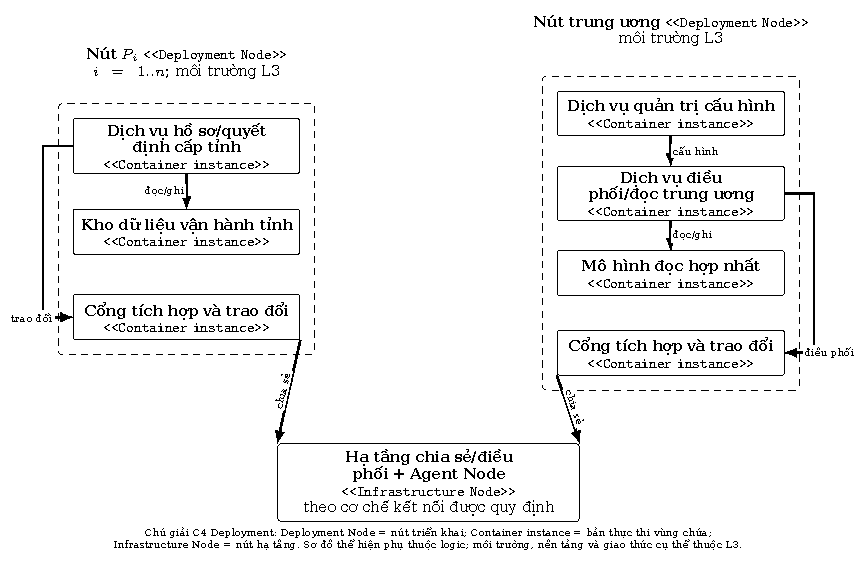
\includegraphics[width=0.94\textwidth]{figure_sources/fig05_c4_deployment_pdist.pdf}
\caption{Cấu hình triển khai logic P-DIST dùng cho stress-test; hạ tầng chia sẻ/điều phối và Agent Node là vai trò kết nối, không phải topology bắt buộc của SRA}
\label{fig:pdist-main}
\end{figure}

Trong ánh xạ này, ``Cổng tích hợp và trao đổi'' là vai trò logic của bộ thích nghi tích hợp. Khi hiện thực hóa trong hệ sinh thái Bộ Khoa học và Công nghệ, vai trò đó phải tương thích với lớp tích hợp, chia sẻ và điều phối của QĐ 1973 (LGSP/LDOP, API Gateway, Agent Node) và cơ chế kết nối qua Nền tảng chia sẻ, điều phối dữ liệu/Agent Node theo NĐ 278 \citep[Mục~III.1.4]{qd1973_2026} \citep[khoản~2 Điều~4; khoản~3 Điều~7]{nd278_2025}. Vì vậy, Hình~\ref{fig:pdist-main} là profile L2 phục vụ đánh giá kiến trúc, không phải sơ đồ triển khai chính thức hoặc cấu hình được các văn bản dẫn chiếu bắt buộc.

Tương tự, góc nhìn an toàn/riêng tư chỉ khóa các bất biến kiến trúc: xác thực theo nguồn phù hợp, ủy quyền theo vai trò và phạm vi, tách đặc quyền tỉnh--trung ương, kiểm soát trường dữ liệu được trao đổi, lưu nguồn gốc/phiên bản và bằng chứng gửi--nhận, cùng trách nhiệm kiểm toán. Các yêu cầu này được dẫn xuất từ NĐ 69, NĐ 278, Luật Bảo vệ dữ liệu cá nhân và NĐ 356 \citep{nd69_2024,nd278_2025,luatbvdlcn2025,nd356_2025}. Chúng không chứng minh rằng một hệ thống chưa triển khai đã đạt cấp độ an toàn thông tin, thông lượng, tính sẵn sàng hay thời gian phục hồi cụ thể; các thuộc tính đó phải được kiểm chứng trên hiện thực hóa thực tế. Ma trận biên tin cậy--kiểm soát chi tiết được cung cấp trong tài liệu bổ trợ.

Cuối cùng, biến thể địa phương được giới hạn ở bước nội bộ, vai trò phối hợp và biểu mẫu phụ trợ; không được thay đổi thẩm quyền, trạng thái quyết định hoặc thời hạn L1, và phải có phiên bản/ngày hiệu lực. Cấu trúc mô hình chung--biến thể địa phương phù hợp với tiền lệ về quy trình cấu hình trong chính quyền đô thị \citep[pp.~486--500]{gottschalk2009municipality}. Đồng thời, địa bàn được dùng để xác định thẩm quyền chứ không làm ranh giới của toàn bộ hệ sinh thái: quan hệ doanh nghiệp--quỹ--chuyên gia--viện/trường cần được lưu xuyên địa bàn \citep[pp.~27--28]{fischer2022}; \citep[pp.~1483--1484]{noak2025}.

%=====================================================================
% 08 — ĐÁNH GIÁ KIẾN TRÚC — bản rút gọn theo hướng bài báo khoa học
%=====================================================================
\section{Đánh giá kiến trúc theo kịch bản}
\label{sec:evaluation}

\subsection{Thiết lập đánh giá và kết quả tổng quát}
\label{subsec:eval-baseline}

B1 là cấu hình ứng viên của SRA theo profile P-DIST trước vòng đánh giá; B0 là một cấu hình tập trung dùng làm đường cơ sở định tính để làm rõ các đánh đổi. Hai cấu hình khác nhau đồng thời ở nhiều quyết định, vì vậy B0 không được dùng như đối chứng thực nghiệm và kết quả không được diễn giải như bằng chứng rằng một topology tốt hơn topology khác. Mười kịch bản SC1--SC10 và rubric ba mức đã trình bày ở Mục~\ref{subsec:scenario-method} được áp dụng trước cho B1, sau đó áp dụng lại cho B1-R sau tinh chỉnh.

Kết quả ban đầu gồm \textbf{2 kịch bản đáp ứng trực tiếp, 7 đáp ứng có điều kiện và 1 rủi ro kiến trúc}. Sau vòng tinh chỉnh, B1-R đạt \textbf{2 đáp ứng trực tiếp, 8 đáp ứng có điều kiện và không còn rủi ro kiến trúc chưa được hấp thụ ở mức thiết kế L2}. Cùng rubric ba mức được áp dụng cho \textbf{B0} như đường cơ sở đối chiếu định tính: B0 đạt \textbf{4 đáp ứng trực tiếp, 4 đáp ứng có điều kiện và 2 rủi ro kiến trúc}. B0 và B1(-R) khác nhau đồng thời ở nhiều quyết định kiến trúc (không chỉ topology), nên kết quả không hỗ trợ suy luận nhân quả cho một quyết định riêng lẻ và không phải một xếp hạng; ý nghĩa của việc đối chiếu được thảo luận ở Mục~\ref{subsec:eval-limitations}. Bảng~\ref{tab:evaluation} giữ toàn bộ mười kịch bản nhưng chỉ trình bày phát hiện có ý nghĩa đối với lập luận kiến trúc; các mã thành phần, quy tắc phù hợp, neo kiến trúc của B0 và phép kiểm tra chi tiết được chuyển sang tài liệu bổ trợ (S12).

{\vjsttablefont
\setlength{\tabcolsep}{2.4pt}
\renewcommand{\arraystretch}{1.02}
\begin{longtable}{@{}>{\raggedright\arraybackslash}p{3.5cm}>{\raggedright\arraybackslash}p{1.75cm}>{\raggedright\arraybackslash}p{1.75cm}>{\raggedright\arraybackslash}p{1.75cm}>{\raggedright\arraybackslash}p{5.25cm}@{}}
\caption{Kết quả stress-test B1, kiểm tra lại B1-R và đối chiếu định tính với đường cơ sở tập trung B0, bằng cùng rubric}
\label{tab:evaluation}\\
\toprule
\textbf{Kịch bản} & \textbf{B0} & \textbf{B1} & \textbf{B1-R} & \textbf{Hàm ý kiến trúc chính} \\
\midrule
\endfirsthead
\multicolumn{5}{c}{\tablename\ \thetable\ -- tiếp theo}\\
\toprule
\textbf{Kịch bản} & \textbf{B0} & \textbf{B1} & \textbf{B1-R} & \textbf{Hàm ý kiến trúc chính} \\
\midrule
\endhead
\bottomrule
\endfoot
SC1. Tỉnh xử lý và quyết định theo thẩm quyền & \textbf{Trực tiếp} & \textbf{Trực tiếp} & \textbf{Trực tiếp} & Biên quyền ghi theo phạm vi thẩm quyền là phù hợp với nghiệp vụ phân cấp, độc lập với topology lưu trữ. \\
SC2. Hai tỉnh khác bước nội bộ nhưng cùng nghĩa vụ pháp lý & \textbf{Trực tiếp} & \textbf{Trực tiếp} & \textbf{Trực tiếp} & Cần tách mô hình nền pháp lý khỏi cấu hình nội bộ có kiểm soát, độc lập với topology lưu trữ. \\
SC3. Quy định thay đổi trạng thái, biểu mẫu hoặc thời hạn & \textbf{Có điều kiện} & \textbf{Có điều kiện} & \textbf{Có điều kiện} & Thay đổi phải đi qua quản trị phiên bản và xử lý hồ sơ đang chạy; B0 chỉ nhẹ hơn ở khâu phát hành hạ tầng, không ở khâu cấu hình theo tỉnh. \\
SC4. Chia sẻ trung ương gián đoạn sau quyết định của tỉnh & \textbf{Rủi ro} & \textbf{Có điều kiện} & \textbf{Có điều kiện} & Xử lý cục bộ và đồng bộ lại chỉ khả thi nếu có kho vận hành tách biệt theo tỉnh (P-DIST); B0 không có tuyến cách ly đó nên gián đoạn trung tâm có thể chặn cả ghi cục bộ. \\
SC5. Trung ương cần ảnh dữ liệu toàn quốc & \textbf{Trực tiếp} & \textbf{Có điều kiện} & \textbf{Có điều kiện} & Mô hình đọc hợp nhất phải công bố nguồn, phiên bản và độ mới; B0 không cần mô hình đọc tách biệt vì đọc trực tiếp trên kho giao dịch. \\
SC6. Định danh doanh nghiệp thay đổi tại nguồn quốc gia & \textbf{Có điều kiện} & \textbf{Có điều kiện} & \textbf{Có điều kiện} & Dữ liệu tham chiếu phải được làm mới và xác minh lại từ nguồn có thẩm quyền; B0 có ít bản tham chiếu cần đồng bộ lại hơn. \\
SC7. Lớp trung ương không sẵn sàng khi tỉnh đang xử lý & \textbf{Rủi ro} & \textbf{Có điều kiện} & \textbf{Có điều kiện} & Khả năng tiếp tục cục bộ phụ thuộc ranh giới rõ giữa bước địa phương và bước bắt buộc dùng dịch vụ ngoài; B0 không có ranh giới vật lý đó nên miền sự cố rộng hơn. \\
SC8. Quan hệ đầu tư/hỗ trợ vượt địa giới & \textbf{Trực tiếp} & \textbf{Có điều kiện} & \textbf{Có điều kiện} & Quan hệ hệ sinh thái phải độc lập với biên thẩm quyền và giữ nguồn cùng thời gian hiệu lực; B0 không cần bước hợp nhất liên kho. \\
SC9. Chuyển phạm vi quản lý từ tỉnh A sang B & \textbf{Có điều kiện} & \textbf{Rủi ro} & \textbf{Có điều kiện} & Biên ghi theo địa bàn là chưa đủ; quyền ghi phải được biểu diễn như một gán quyền có hiệu lực theo thời gian. B0 vẫn cần chuyển giao đó nhưng không cần đồng bộ chéo hai kho vật lý. \\
SC10. Các tỉnh nâng lược đồ/quy trình lệch thời điểm & \textbf{Có điều kiện} & \textbf{Có điều kiện} & \textbf{Có điều kiện} & Kiến trúc cần quản trị tương thích phiên bản và quy tắc chuyển đổi minh thị; ở B0 chỉ còn rủi ro lệch phiên bản cấu hình quy trình, không còn lệch phiên bản lược đồ liên kho. \\
\end{longtable}
}

\subsection{Phát hiện dẫn tới tinh chỉnh B1-R}
\label{subsec:eval-results}

Phát hiện quan trọng nhất là SC9. B1 đã tách quyền ghi theo địa bàn nhưng chưa mô hình hóa việc quyền đó thay đổi theo thời gian. Khi phạm vi quản lý một chủ thể chuyển từ tỉnh A sang tỉnh B, chỉ di chuyển hoặc sao chép dữ liệu không bảo đảm rằng tại cùng một thời điểm chỉ một phía có quyền thay đổi trạng thái, cũng không bảo toàn đầy đủ lịch sử và nguồn gốc của quyết định. Vòng DSR vì vậy tinh chỉnh nguyên tắc quyền ghi của B1-R thành một quan hệ có phạm vi, thời gian hiệu lực và bằng chứng chuyển giao, với bất biến chỉ một writer đang hiệu lực cho cùng phạm vi. Chi tiết biểu diễn và giao thức chuyển quyền được giữ trong tài liệu bổ trợ vì chúng là phương án L2 cần được kiểm chứng khi hiện thực hóa, không phải đặc tả bắt buộc của SRA.

SC10 làm lộ một vấn đề khác: phiên bản của hợp đồng dữ liệu và quy trình không thể giả định được nâng đồng thời ở mọi tỉnh. B1-R do đó bổ sung cửa sổ tương thích, phiên bản tối thiểu còn hỗ trợ, ghim phiên bản cho hồ sơ đang xử lý và quy tắc chuyển đổi minh thị. Tinh chỉnh này không thay đổi mục tiêu chức năng của SRA nhưng làm rõ điều kiện để các nút có thể tiến hóa độc lập mà vẫn duy trì liên thông và khả năng đọc dữ liệu lịch sử.

Hai phát hiện trên cho thấy giá trị của phép đánh giá nằm ở việc \emph{làm lộ điểm chưa đầy đủ và buộc sửa artefact}, chứ không chỉ xác nhận kiến trúc đã xây dựng. Chuỗi B1 $\rightarrow$ stress-test $\rightarrow$ tinh chỉnh $\rightarrow$ B1-R vì vậy đóng vai trò vòng đánh giá--thiết kế của nghiên cứu. Việc SC9 chuyển từ \textsc{rủi ro} sang \textsc{đáp ứng có điều kiện} chỉ cho biết khoảng trống đã được hấp thụ ở cấp thiết kế; tám kịch bản còn ở mức có điều kiện vẫn đòi hỏi bằng chứng hiện thực hóa.

\subsection{Diễn giải và giới hạn của bằng chứng đánh giá}
\label{subsec:eval-limitations}

Chấm B0 bằng đúng rubric ba mức trên cả mười kịch bản (lập luận theo từng kịch bản ở S12 tài liệu bổ trợ) cho kết quả \textbf{4 đáp ứng trực tiếp, 4 đáp ứng có điều kiện và 2 rủi ro kiến trúc}. B0 đáp ứng trực tiếp hoặc tốt hơn B1-R đúng ở các kịch bản không phụ thuộc việc cách ly vật lý theo tỉnh: SC1/SC2 vì cơ chế gán quyền ghi và quản trị cấu hình quy trình vốn topology-độc lập; SC5/SC8 vì một kho tập trung không cần một mô hình đọc hoặc bước hợp nhất quan hệ liên kho riêng; và một phần SC9 vì chuyển quyền ghi không cần giao thức đồng bộ hay di chuyển dữ liệu vật lý giữa hai kho. Ngược lại, B0 rơi xuống mức rủi ro kiến trúc đúng ở hai kịch bản gắn với cô lập miền sự cố khi lớp trung ương gián đoạn (SC4, SC7): vì B0 không tách kho vận hành theo tỉnh, một gián đoạn ở lớp trung tâm có thể chặn cả khả năng tỉnh tự ghi quyết định cục bộ, không chỉ chặn bước đồng bộ như ở P-DIST. Đây là đánh đổi cố hữu của phương án ``kho tập trung đa tenant'' tại điểm biến thiên VP7 -- đã được ghi nhận sẵn trong đánh đổi của AD01 -- chứ không phải một khoảng trống mới đòi hỏi sửa lại lõi ổn định.

Kết quả cho thấy không có cấu hình nào ưu việt đồng loạt: B0 không tệ hơn B1-R một cách hệ thống, và P-DIST/B1-R cũng không ưu việt hơn B0 một cách hệ thống; mỗi cấu hình bộc lộ một hồ sơ đánh đổi khác nhau tùy kịch bản. \textbf{Điểm cần nhấn mạnh là B0 và B1(-R) khác nhau đồng thời ở nhiều quyết định kiến trúc, không chỉ ở topology lưu trữ} -- lựa chọn topology kéo theo khác biệt cả ở cơ chế mô hình đọc, hợp nhất quan hệ và ranh giới miền sự cố. Vì vậy phép đối chiếu này \textbf{không cho phép suy luận nhân quả về giá trị của một quyết định kiến trúc riêng lẻ} và không phải một xếp hạng hiệu năng hay chi phí; đây chỉ là đối chiếu đánh đổi định tính ở mức kiến trúc.

Phép đánh giá là \textbf{kiểm chứng kiến trúc theo kịch bản trước triển khai} (\textit{scenario-based architecture verification/stress-test}). Các kịch bản được xây dựng và chấm bởi cùng nhóm tác giả; nghiên cứu chưa có prototype vận hành, tải thực, phép đo độ trễ/tính sẵn sàng, thời gian phục hồi, chi phí hay đánh giá người dùng. Vì vậy, kết quả chỉ chứng minh mức đầy đủ và tính nhất quán tương đối của artefact dưới các kịch bản đã chọn, không chứng minh một topology tốt hơn topology khác. Bằng chứng tiếp theo cần đến từ nguyên mẫu và các phép thử có thể lặp lại đối với chuyển quyền ghi, tương thích/nâng cấp, liên thông, phục hồi và an toàn.

%=====================================================================
% 09 — BÀN LUẬN — scientific-paper compression
%=====================================================================
\section{Bàn luận}
\label{sec:discussion}

\subsection{Ý nghĩa của đóng góp kiến trúc}
\label{subsec:delta}

Đóng góp của nghiên cứu không nằm ở một topology triển khai cụ thể mà ở cách SRA tách \emph{lõi ổn định} khỏi \emph{điểm biến thiên}. Lõi ổn định bảo toàn quyền ghi theo thẩm quyền, nguồn gốc và hiệu lực dữ liệu, cùng trách nhiệm liên thông; còn bố trí kho dữ liệu, cơ chế tích hợp và chi tiết quy trình địa phương được để ở lớp biến thiên. Cách tách này cho phép thay đổi tổ chức hoặc công nghệ mà không phải diễn giải lại các nghĩa vụ nền tảng.

Mô hình thẩm quyền theo \emph{nhóm thuộc tính} là điểm khác biệt thứ hai: định danh pháp lý, trạng thái chuyên ngành, bằng chứng ngoài hệ thống và dữ liệu dẫn xuất có thể thuộc các nguồn có thẩm quyền khác nhau. Nhờ đó, nền tảng chuyên ngành không trở thành một nguồn pháp lý song song. Chuỗi truy vết từ nguồn tới quyết định kiến trúc đồng thời vận hành hóa yêu cầu về tính phù hợp kiến trúc trước đầu tư tại Khung kiến trúc số của Bộ KH\&CN \citep{qd1973_2026}; giá trị của nó nằm ở khả năng giải thích vì sao một quyết định tồn tại và phần nào phải xem xét lại khi nguồn thay đổi, thay vì ở số lượng mã truy vết nội bộ.

\subsection{Các nguyên tắc thiết kế có khả năng khái quát và đối sánh với khung hiện hành}
\label{subsec:design-principles}

Từ hai đóng góp kiến trúc và các phát hiện của stress-test, nghiên cứu rút ra ba nguyên tắc thiết kế ở mức khái quát. Các nguyên tắc này không được trình bày như quy luật phổ quát; chúng là \emph{design knowledge} có điều kiện, có khả năng chuyển giao cho các nền tảng khu vực công có phân cấp thẩm quyền, nhiều nguồn dữ liệu có thẩm quyền và yêu cầu liên thông đa cấp tương tự. Cơ sở kiến trúc của các quan sát này đã được lập luận ở Mục~\ref{subsec:scope-viewpoints}--\ref{subsec:arch-decisions}; phần dưới đây khái quát chúng thành design knowledge có thể chuyển giao.

\textbf{P1 -- Phân rã thẩm quyền theo nhóm thuộc tính--phạm vi--thời gian.} Nguồn có thẩm quyền và quyền ghi nên được xác định theo từng nhóm thuộc tính, phạm vi nghiệp vụ và khoảng hiệu lực thay vì gán toàn bộ thực thể cho một CSDL hoặc một cơ quan. Nguyên tắc này cho phép định danh pháp lý, trạng thái chuyên ngành và dữ liệu dẫn xuất cùng tồn tại mà không tạo các nguồn pháp lý song song.

\textbf{P2 -- Lõi pháp lý ổn định, biến thể vận hành có kiểm soát.} Thẩm quyền, trạng thái quyết định, nguồn pháp lý và thời hạn bắt buộc thuộc stable core; bước xử lý nội bộ, vai trò phối hợp, biểu mẫu phụ trợ và cấu hình địa phương có thể biến thiên nếu được version hóa và không làm thay đổi lõi này. Cách tách đó cho phép thích nghi tổ chức mà không phải tái diễn giải nghĩa vụ pháp lý mỗi khi quy trình vận hành thay đổi.

\textbf{P3 -- Liên thông độc lập topology nhưng không độc lập provenance.} Biên thẩm quyền, trách nhiệm liên thông và nguồn gốc dữ liệu phải được bảo toàn bất kể hệ thống dùng kho tập trung, phân vùng hay phân tán. Bản sao, mô hình đọc và dữ liệu tổng hợp chỉ có thể thay đổi nơi lưu và cách truy cập; chúng vẫn phải giữ nguồn, phiên bản, thời điểm hiệu lực và bằng chứng trao đổi để không bị diễn giải như nguồn quyết định gốc.

Để làm rõ mức độ mà SRA đã được neo vào các khung mới hiện hành, Bảng~\ref{tab:conformance-current} đối sánh trực tiếp yêu cầu kiến trúc với biểu hiện trong artefact. Bảng này là bằng chứng truy vết/conformance ở mức thiết kế, không phải chứng nhận rằng một hệ thống chưa triển khai đã tuân thủ đầy đủ mọi yêu cầu kỹ thuật và an toàn.

{\vjsttablefont
\renewcommand{\arraystretch}{1.02}
\setlength{\tabcolsep}{2.5pt}
\begin{table}[H]
\centering
\caption{Đối sánh SRA với các khung kiến trúc, dữ liệu và liên thông hiện hành}
\label{tab:conformance-current}
\begin{tabularx}{\textwidth}{@{}p{3.0cm}XXX@{}}
\toprule
\textbf{Nguồn/vị trí} & \textbf{Yêu cầu kiến trúc} & \textbf{Biểu hiện trong SRA} & \textbf{Bằng chứng} \\
\midrule
QĐ 3090/QĐ-BKHCN, Điều 1 \citep{qd3090_2025}; QĐ 292/QĐ-BKHCN, Chương 2 Mục II; Chương 3 Mục II.6--7 \citep{qd292_2025} & Nền tảng chuyên ngành phải đặt trong hệ quy chiếu kiến trúc số quốc gia, kiểm tra theo các mô hình tham chiếu nghiệp vụ, dữ liệu, ứng dụng, công nghệ, ATTT và dùng lớp tích hợp/chia sẻ quốc gia, cấp bộ/tỉnh, thay vì hình thành kiến trúc biệt lập. & Hình~\ref{fig:dinhvi} định vị SRA giữa khung số, dữ liệu và nghiệp vụ; stable core/variation tách nghĩa vụ ổn định khỏi lựa chọn công nghệ; các góc nhìn năng lực--ứng dụng, dữ liệu--thẩm quyền và container tách ranh giới trách nhiệm; trao đổi liên cơ quan đi qua lớp tích hợp thay vì điểm--điểm tùy ý. & Hình~\ref{fig:dinhvi}; Hình~\ref{fig:ranhgioi}; Mục~\ref{subsec:phanlop}; Mục~\ref{sec:interop}. \\
QĐ 2439/QĐ-TTg \citep{qd2439_2025}; NĐ 278, khoản 2,4 Điều 4; khoản 2 Điều 5; khoản 2--3 Điều 7 \citep{nd278_2025} & Một nguồn tin cậy cho dữ liệu chủ; chia sẻ bắt buộc qua Nền tảng chia sẻ, điều phối; Agent Node tại bộ/địa phương. & Thẩm quyền được xác định theo nhóm thuộc tính; bản sao giữ provenance/phiên bản; cổng tích hợp của SRA thích nghi với hạ tầng chia sẻ/điều phối. & Hình~\ref{fig:pdist-main}; Mục~\ref{sec:data}--\ref{sec:interop}. \\
QĐ 1973/QĐ-BKHCN, Mục II.1(b), III.1.4, III.3.3 \citep{qd1973_2026} & Thu thập một lần, một nguồn dữ liệu gốc; đồng bộ qua nền tảng tích hợp của Bộ; dữ liệu tổ chức/doanh nghiệp nhận từ nguồn quốc gia. & SRA không tạo master định danh doanh nghiệp song song; tỉnh quản trị trạng thái chuyên ngành theo thẩm quyền; Hình~\ref{fig:pdist-main} ánh xạ logic tới LGSP/LDOP--Agent Node. & Mục~\ref{subsec:phanlopdulieu}; Mục~\ref{subsec:v5v6}. \\
NĐ 268/2025/NĐ-CP, Điều 48; khoản 2 Điều 66 \citep{nd268_2025} & Thẩm quyền nghiệp vụ chủ yếu ở cấp tỉnh nhưng có nghĩa vụ cập nhật/thông báo liên cấp và thời hạn luật định. & Quyền ghi bám thẩm quyền có hiệu lực; trung ương đọc/tổng hợp; sự kiện trao đổi giữ bằng chứng gửi--nhận và không chuyển 15 ngày thành API SLA. & Mục~\ref{subsec:phanlopdulieu}; Mục~\ref{subsec:sla}. \\
NĐ 69 \citep{nd69_2024}; Luật Bảo vệ dữ liệu cá nhân \citep{luatbvdlcn2025}; NĐ 356 \citep{nd356_2025} & Định danh/xác thực, phân quyền theo phạm vi, tối thiểu hóa và bảo vệ dữ liệu, truy vết/kiểm toán. & Xác thực theo nguồn phù hợp; tách đặc quyền tỉnh--trung ương; kiểm soát trường trao đổi; lưu provenance, version và audit evidence. & Mục~\ref{subsec:v5v6}; tài liệu bổ trợ. \\
\bottomrule
\end{tabularx}
\end{table}
}

Đối sánh cho thấy SRA đã có các điểm neo rõ vào hệ quy chiếu hiện hành ở mức nghiệp vụ, dữ liệu và liên thông. Tuy nhiên, các hàng trên không khóa công nghệ và không thay thế thẩm định triển khai: sản phẩm CSDL, giao thức, cấu hình bảo mật, chỉ tiêu hiệu năng và bằng chứng kết nối thực tế vẫn thuộc giai đoạn hiện thực hóa/kiểm thử. Các nguồn dự thảo chỉ tiếp tục được dùng như tín hiệu chẩn đoán, không được đưa vào bảng như nghĩa vụ bắt buộc.

\subsection{Trade-off, P-DIST và khả năng khái quát}
\label{subsec:distributed-discussion}

Kết quả kịch bản không cho thấy P-DIST ưu việt hơn kiến trúc tập trung. P-DIST hỗ trợ biên vận hành địa phương và cô lập một số lỗi, nhưng làm tăng yêu cầu phối hợp phiên bản, tổng hợp toàn quốc và chuyển quyền ghi; phương án tập trung thuận lợi hơn cho phát hành thay đổi và tạo ảnh đọc toàn quốc. Vì vậy, P-DIST chỉ là một cấu hình dùng để kiểm tra xem các bất biến của SRA có được bảo toàn dưới phân tán hay không, không phải khuyến nghị mặc định ``mỗi tỉnh một kho vật lý''.

Hai phát hiện SC9--SC10 có ý nghĩa rộng hơn cấu hình này. SC9 cho thấy thẩm quyền ghi là quan hệ có hiệu lực theo thời gian, không chỉ là ánh xạ tĩnh theo địa bàn; SC10 cho thấy một SRA dùng chung phải chịu được giai đoạn các đơn vị vận hành khác phiên bản. B1-R vì thế bổ sung chuyển quyền và quản trị tương thích ở mức kiến trúc, trong khi chi tiết hiện thực hóa vẫn phải được kiểm chứng bằng nguyên mẫu.

Khả năng chuyển giao còn nằm ở việc tách biên thẩm quyền khỏi biên hệ sinh thái. Các nghiên cứu cho thấy quan hệ khởi nghiệp và đầu tư có thể vượt địa giới hành chính \citep[pp.~28, 32]{fischer2022}; \citep[pp.~1483--1484]{noak2025}. Do đó, địa bàn phù hợp để xác định thẩm quyền và phạm vi xử lý nhưng không nên là ranh giới bắt buộc của quan hệ doanh nghiệp--quỹ--chuyên gia--viện/trường. Nguyên tắc này có thể áp dụng cho các nền tảng công khác có xử lý phân quyền nhưng dữ liệu/liên thông dùng chung; topology cụ thể vẫn phải được lựa chọn theo thẩm quyền, miền sự cố và yêu cầu đồng bộ của từng hệ thống.

\subsection{Giới hạn nghiên cứu}
\label{subsec:limits-transfer}

Bằng chứng hiện tại dừng ở \emph{scenario-based architecture verification} trước triển khai. Bộ mười kịch bản đã phát hiện khoảng trống thiết kế và dẫn tới B1-R, nhưng không chứng minh bộ kịch bản là đầy đủ; việc xây dựng và chấm kịch bản vẫn do nhóm tác giả thực hiện. Các nguồn dự thảo chỉ có vai trò chẩn đoán và không tạo nghĩa vụ bắt buộc cho SRA.

Nghiên cứu chưa cung cấp bằng chứng thực nghiệm về hiệu năng, tính sẵn sàng, an toàn, phục hồi hoặc liên thông vận hành. Bước tiếp theo vì vậy là xây dựng nguyên mẫu và kiểm thử lặp lại đối với chuyển quyền ghi, nâng cấp lệch phiên bản, gián đoạn kết nối, trao đổi qua hạ tầng dùng chung và các thuộc tính chất lượng đo được. Chỉ khi đó mới có thể xác nhận các cơ chế L2 chuyển thành hành vi triển khai đúng với chi phí vận hành chấp nhận được.

%=====================================================================
% 10 — KẾT LUẬN — scientific-paper compression
%=====================================================================
\section{Kết luận}
\label{sec:conclusion}

Bài báo đề xuất một kiến trúc tham chiếu phần mềm tỉnh--trung ương cho nền tảng quản lý DN KH\&CN và DN KNST, trong đó quyền xử lý nghiệp vụ chủ yếu thuộc cấp tỉnh nhưng dữ liệu, liên thông và tổng hợp phải bảo đảm tính thống nhất ở cấp Bộ/quốc gia. Đóng góp chính là một mô hình \emph{gán quyền ghi theo phạm vi thẩm quyền và thời gian hiệu lực} -- với máy trạng thái chuyển giao và bất biến single-active-writer -- tổng quát hóa được cho các nền tảng chính phủ đa cấp khác, không riêng miền DN KH\&CN/DN KNST; cách tổ chức \emph{lõi ổn định} và \emph{điểm biến thiên} của SRA; ranh giới trách nhiệm liên thông; và chuỗi truy vết cho phép nối căn cứ nguồn với quyết định kiến trúc và tiêu chí đánh giá. SRA không bắt buộc một topology lưu trữ; P-DIST chỉ được dùng như một cấu hình để thử thách các bất biến kiến trúc dưới điều kiện phân tán. Ba nguyên tắc thiết kế được rút ra ở mức khái quát là: phân rã thẩm quyền theo nhóm thuộc tính--phạm vi--thời gian; tách lõi pháp lý ổn định khỏi biến thể vận hành có kiểm soát; và duy trì provenance/liên thông độc lập với topology lưu trữ.

Mười kịch bản cho thấy ứng viên ban đầu còn hai khoảng trống quan trọng: chuyển quyền ghi phải được biểu diễn theo thời gian và kiến trúc phải chịu được giai đoạn các đơn vị vận hành khác phiên bản. Sau khi hai vấn đề này được hấp thụ vào B1-R, hậu kiểm bằng cùng rubric cho kết quả 2 kịch bản đáp ứng trực tiếp, 8 kịch bản đáp ứng có điều kiện và không còn rủi ro kiến trúc chưa được hấp thụ ở mức L2 trong bộ kịch bản hiện tại. Kết quả này là \emph{scenario-based architecture verification} trước triển khai, không phải bằng chứng thực nghiệm về một hệ thống vận hành. Bước tiếp theo là xây dựng nguyên mẫu và kiểm thử lặp lại đối với chuyển quyền ghi, nâng cấp lệch phiên bản, liên thông, phục hồi, an toàn và các thuộc tính chất lượng đo được.


% Không dựng mục Lời cảm ơn khi chưa có thông tin tài trợ/hỗ trợ được tác giả xác nhận.
% Polyglossia có thể đặt lại tên mục tài liệu khi bắt đầu document; khóa lại ngay trước bibliography.
\renewcommand{\refname}{TÀI LIỆU THAM KHẢO}
%=====================================================================
% TÀI LIỆU THAM KHẢO — trình bày tiếng Anh theo quy định VJST-MOST.
% Thứ tự bibitem phải theo lần xuất hiện đầu tiên trong thân bài.
%=====================================================================
\begin{thebibliography}{99}
\setlength{\itemsep}{0.35em}

\bibitem{nd268_2025}
Government of Vietnam (2025), \textit{Decree No. 268/2025/ND-CP Detailing and Guiding a Number of Articles of the Law on Science, Technology and Innovation Concerning Innovation, Science, Technology and Innovation Activities in Enterprises, Recognition of Innovation Centers and Innovative Startups, and Startup Ecosystem Infrastructure}, 69pp, \url{https://vanban.chinhphu.vn/?classid=1&docid=215663&orggroupid=2&pageid=27160}, accessed 9 August 2026 (in Vietnamese).

\bibitem{nhom_bai1}
N.D. Quang, N.H. Cuong (2026), ``Digital governance platform for the innovative startup and science - technology enterprise ecosystem: Insights from Decree No. 268/2025/ND-CP and Korean's experience'', \textit{Journal of Science and Technology Policy and Management}, \textbf{15(2)}, pp.45--68, \url{https://vietnamstijournal.net/index.php/JSTPM/article/view/534}, accessed 10 August 2026 (in Vietnamese).

\bibitem{angelov2012}
S. Angelov, P. Grefen, D. Greefhorst (2012), ``A framework for analysis and design of software reference architectures'', \textit{Information and Software Technology}, \textbf{54(4)}, pp.417--431, DOI: 10.1016/j.infsof.2011.11.009.

\bibitem{iso42010_2022}
ISO/IEC/IEEE (2022), \textit{ISO/IEC/IEEE 42010:2022 Software, Systems and Enterprise---Architecture Description}, 2nd ed., International Organization for Standardization, 62pp, \url{https://www.iso.org/standard/74393.html}, accessed 9 August 2026.

\bibitem{manikas2013}
K. Manikas, K.M. Hansen (2013), ``Software ecosystems---A systematic literature review'', \textit{Journal of Systems and Software}, \textbf{86(5)}, pp.1294--1306, DOI: 10.1016/j.jss.2012.12.026.

\bibitem{wang2021}
P. Wang (2021), ``Connecting the parts with the whole: Toward an information ecology theory of digital innovation ecosystems'', \textit{MIS Quarterly}, \textbf{45(1)}, pp.397--422, DOI: 10.25300/MISQ/2021/15864.

\bibitem{winkler2010}
S. Winkler, J. von Pilgrim (2010), ``A survey of traceability in requirements engineering and model-driven development'', \textit{Software \& Systems Modeling}, \textbf{9}, pp.529--565, DOI: 10.1007/s10270-009-0145-0.

\bibitem{kosenkov2025}
O. Kosenkov, P. Elahidoost, T. Gorschek, et al. (2025), ``Systematic mapping study on requirements engineering for regulatory compliance of software systems'', \textit{Information and Software Technology}, \textbf{178}, Article 107622, DOI: 10.1016/j.infsof.2024.107622.

\bibitem{qd3090_2025}
Ministry of Science and Technology of Vietnam (2025), \textit{Decision No. 3090/QD-BKHCN Promulgating the National Overall Digital Architecture Framework}, issued 8 October 2025 (in Vietnamese).

\bibitem{qd2439_2025}
Prime Minister of Vietnam (2025), \textit{Decision No. 2439/QD-TTg Promulgating the National Data Architecture Framework, National Data Governance and Management Framework, and Common Data Dictionary (Version 1.0)}, issued 4 November 2025, \url{https://vanban.chinhphu.vn/?classid=0&docid=215785&pageid=27160}, accessed 9 August 2026 (in Vietnamese).

\bibitem{qd1973_2026}
Ministry of Science and Technology of Vietnam (2026), \textit{Decision No. 1973/QD-BKHCN Promulgating the Data Architecture Framework and Data Governance and Management Framework of the Ministry of Science and Technology (Version 1.0)}, issued 31 March 2026 (in Vietnamese).

\bibitem{eif2017}
European Commission (2017), \textit{New European Interoperability Framework: Promoting Seamless Services and Data Flows for European Public Administrations}, Publications Office of the European Union, 48pp, DOI: 10.2799/78681.

\bibitem{fischer2022}
B. Fischer, D. Meissner, N. Vonortas, et al. (2022), ``Spatial features of entrepreneurial ecosystems'', \textit{Journal of Business Research}, \textbf{147}, pp.27--36, DOI: 10.1016/j.jbusres.2022.04.018.

\bibitem{noak2025}
N.V. Noak, L. Christian (2025), ``Exploring spatial network structures in entrepreneurial ecosystems: A network and clustering analysis of global venture funding flows'', \textit{Small Business Economics}, \textbf{65}, pp.1483--1500, DOI: 10.1007/s11187-025-01029-y.

\bibitem{oasis_soaraf2012}
P. Brown, J.A. Estefan, K. Laskey, et al. (eds.) (2012), \textit{Reference Architecture Foundation for Service Oriented Architecture Version 1.0}, OASIS Committee Specification 01, 118pp, \url{https://docs.oasis-open.org/soa-rm/soa-ra/v1.0/cs01/soa-ra-v1.0-cs01.pdf}, accessed 9 August 2026.

\bibitem{knodel2016}
J. Knodel, K. Manikas (2016), ``Towards reference architectures as an enabler for software ecosystems'', in \textit{Proceedings of the 10th European Conference on Software Architecture Workshops (ECSAW 2016)}, Article 26, Association for Computing Machinery, DOI: 10.1145/2993412.3003387.

\bibitem{kruize2016}
J.W. Kruize, J. Wolfert, H. Scholten, et al. (2016), ``A reference architecture for Farm Software Ecosystems'', \textit{Computers and Electronics in Agriculture}, \textbf{125}, pp.12--28, DOI: 10.1016/j.compag.2016.04.011.

\bibitem{breaux2006}
T.D. Breaux, M.W. Vail, A.I. Ant\'on (2006), ``Towards regulatory compliance: Extracting rights and obligations to align requirements with regulations'', in \textit{14th IEEE International Requirements Engineering Conference (RE'06)}, pp.49--58, DOI: 10.1109/RE.2006.68.

\bibitem{gallagher2000}
B.P. Gallagher (2000), \textit{Using the Architecture Tradeoff Analysis Method to Evaluate a Reference Architecture: A Case Study}, Technical Note CMU/SEI-2000-TN-007, Software Engineering Institute, Carnegie Mellon University, 25pp, \url{https://www.sei.cmu.edu/documents/1960/2000_004_001_13679.pdf}, accessed 9 August 2026.

\bibitem{euact2024}
European Parliament, Council of the European Union (2024), \textit{Regulation (EU) 2024/903 of 13 March 2024 Laying Down Measures for a High Level of Public Sector Interoperability Across the Union (Interoperable Europe Act)}, Official Journal of the European Union, L series, 26pp, \url{https://eur-lex.europa.eu/eli/reg/2024/903/oj}, accessed 9 August 2026.

\bibitem{qd292_2025}
Ministry of Science and Technology of Vietnam (2025), \textit{Decision No. 292/QD-BKHCN Promulgating the Vietnam Digital Government Architecture Framework, Version 4.0}, issued 25 March 2025 (in Vietnamese).

\bibitem{nd278_2025}
Government of Vietnam (2025), \textit{Decree No. 278/2025/ND-CP on Mandatory Data Connection and Sharing Among Agencies in the Political System}, issued 22 October 2025, \url{https://vanban.chinhphu.vn/?docid=215682&pageid=27160}, accessed 9 August 2026 (in Vietnamese).

\bibitem{nd69_2024}
Government of Vietnam (2024), \textit{Decree No. 69/2024/ND-CP on Electronic Identification and Authentication}, issued 25 June 2024, \url{https://vanban.chinhphu.vn/?classid=1&docid=210491&pageid=27160}, accessed 9 August 2026 (in Vietnamese).

\bibitem{nd169_2025}
Government of Vietnam (2025), \textit{Decree No. 169/2025/ND-CP on Science, Technology and Innovation Activities and Data Products and Services}, issued 30 June 2025, \url{https://vanban.chinhphu.vn/?classid=0&docid=214306&pageid=27160}, accessed 9 August 2026 (in Vietnamese).

\bibitem{luatbvdlcn2025}
National Assembly of Vietnam (2025), \textit{Law on Personal Data Protection No. 91/2025/QH15}, adopted 26 June 2025, \url{https://vanban.chinhphu.vn/?classid=1&docid=214590&pageid=27160&typegroup=}, accessed 9 August 2026 (in Vietnamese).

\bibitem{nd356_2025}
Government of Vietnam (2025), \textit{Decree No. 356/2025/ND-CP Detailing a Number of Articles and Measures for Implementing the Law on Personal Data Protection}, issued 31 December 2025, \url{https://vanban.chinhphu.vn/?classid=1&docid=216387&pageid=27160}, accessed 9 August 2026 (in Vietnamese).

\bibitem{luatkhcndmst2025}
National Assembly of Vietnam (2025), \textit{Law on Science, Technology and Innovation No. 93/2025/QH15}, adopted 27 June 2025, \url{https://vanban.chinhphu.vn/?pageid=27160&docid=214603}, accessed 20 August 2026 (in Vietnamese).

\bibitem{qd1762_2025}
Ministry of Science and Technology of Vietnam (2025), \textit{Decision No. 1762/QD-BKHCN Promulgating the Catalogue of Specialised Databases Under the Management of the Ministry of Science and Technology}, issued 16 July 2025 (in Vietnamese).

\bibitem{luatdulieu2024}
National Assembly of Vietnam (2024), \textit{Data Law No. 60/2024/QH15}, adopted 30 November 2024, \url{https://vanban.chinhphu.vn/?classid=1&docid=212488&pageid=27160&typegroupid=3}, accessed 9 August 2026 (in Vietnamese).

\bibitem{hevner2004}
A.R. Hevner, S.T. March, J. Park, et al. (2004), ``Design science in information systems research'', \textit{MIS Quarterly}, \textbf{28(1)}, pp.75--105.

\bibitem{peffers2007}
K. Peffers, T. Tuunanen, M.A. Rothenberger, et al. (2007), ``A design science research methodology for information systems research'', \textit{Journal of Management Information Systems}, \textbf{24(3)}, pp.45--77, DOI: 10.2753/MIS0742-1222240302.

\bibitem{tyree2005}
J. Tyree, A. Akerman (2005), ``Architecture decisions: Demystifying architecture'',
\textit{IEEE Software}, \textbf{22(2)}, pp.19--27, DOI: 10.1109/MS.2005.27.

\bibitem{c4model2026}
S. Brown (n.d.), ``The C4 model for visualising software architecture'', official C4 model website, \url{https://c4model.com/}, accessed 9 August 2026.

\bibitem{archimate32_2023}
The Open Group (2022), \textit{ArchiMate\textsuperscript{\textregistered} 3.2 Specification}, Version 3.2, released October 2022, \url{https://www.opengroup.org/archimate-licensed-downloads}, accessed 9 August 2026.

\bibitem{gottschalk2009municipality}
F. Gottschalk, T.A.C. Wagemakers, M.H. Jansen-Vullers, et al. (2009), ``Configurable process models: Experiences from a municipality case study'', in P. Eck, J. Gordijn, R. Wieringa (eds.), \textit{Advanced Information Systems Engineering}, Lecture Notes in Computer Science, Vol. 5565, Springer, pp.486--500, DOI: 10.1007/978-3-642-02144-2\_38.

\bibitem{sheth1990}
A.P. Sheth, J.A. Larson (1990), ``Federated database systems for managing distributed, heterogeneous, and autonomous databases'',
\textit{ACM Computing Surveys}, \textbf{22(3)}, pp.183--236, DOI: 10.1145/96602.96604.

\bibitem{duthao_khungtc}
National Agency for Technology Entrepreneurship and Commercialization, Ministry of Science and Technology of Vietnam (2026), \textit{Draft Decision on the Temporary Promulgation of Data Standards, Data Standardisation Rules and Specialised Data Catalogues for Science and Technology Enterprises and Innovative Startups}, draft version reviewed 8 August 2026 (in Vietnamese).

\end{thebibliography}

\end{document}
